% ====================================================================================
\chapter{序列建模：从RNN到Transformer}
% ====================================================================================

\section*{Attention Is All You Need}

\sidenoteplain{2017年Google团队发表“Attention Is All You Need”，提出Transformer，彻底改变了NLP。论文标题模仿Beatles的歌“All You Need Is Love”。这个架构成为GPT、BERT、ChatGPT的基础。}

ChatGPT、GPT-4、Claude——这些震惊世界的AI系统都基于同一个架构：\textbf{Transformer}。为什么它能取代统治自然语言处理（NLP）十年的循环神经网络（RNN）？

本章我们将从两个视角回答这个问题。优化视角问的是：为什么RNN的梯度会消失或爆炸？信息论视角问的是：为什么RNN会“遗忘”长距离信息？两个问题的答案指向同一个根源。然后，我们将从零开始构建Transformer，理解它的每一个组件。

\vspace{0.3cm}
\noindent\textit{为什么一个只有几百万参数的 RNN 记不住 50 个词之前的信息？为什么“注意力”这个看似工程化的技巧，会和第4章的最大熵原理长得一模一样？为什么 Transformer 要给残差连接留一条“高速公路”？}

\begin{quote}
\textbf{本章目标}：把序列建模看成“序列损失 + 隐状态递推约束”的拉格朗日问题。你会发现 RNN 的梯度消失就是乘子 $\lambda_t$（隐状态的影子价格）沿时间指数折损，LSTM 的门控和 Transformer 的残差流都是在保护这个影子价格；而注意力的 softmax 则是第4章最大熵原理的直接产物。读完本章，Q、K、V、缩放、多头、位置编码、残差——都不再是“设计出来的”，而是从约束里自然涌现的。
\end{quote}

\begin{tcolorbox}[colback=green!5, colframe=green!60!black, title=学完这章，你将能够...]
\begin{itemize}
    \item 分析RNN为什么会梯度消失，LSTM如何缓解
    \item 手算Self-Attention的输出（给定Q、K、V矩阵）
    \item 解释为什么Transformer能处理长序列
    \item 用PyTorch实现一个简化版Transformer块
    \item 理解GPT、BERT等大模型的架构差异
\end{itemize}
\end{tcolorbox}

% ====================================================================================
\section{RNN：序列建模的第一次尝试}
% ====================================================================================

在理解Transformer之前，我们需要先理解它的前辈——循环神经网络（Recurrent Neural Network, RNN）。
\storynote{Sepp Hochreiter}{1991年，慕尼黑工大的硕士生 Hochreiter 在 Schmidhuber 指导下写出一篇德文论文，第一次从数学上解释了 RNN 的梯度消失；六年后两人提出 LSTM。这篇论文直到 2000 年代才被英语世界广泛引用——“Attention Is All You Need”其实是在回答他 26 年前提出的问题。}

% ------------------------------------------------------------------------------------
\subsection{序列建模作为约束优化问题}
% ------------------------------------------------------------------------------------

序列数据的特点是每一步都依赖于之前的历史。我们要回答的第一个问题是：这种依赖应该怎样写进优化问题？让我们用熟悉的约束优化框架来理解序列建模——答案是把“依赖历史”写成一条约束。

\begin{keyidea}[序列模型的统一形式]
所有序列模型都可以写成以下约束优化问题：
\begin{equation}
    \begin{aligned}
        \min_{\{h_t\}, \theta} \quad & J = \sum_{t=1}^{T} \ell(h_t, y_t) \\
        \text{s.t.} \quad & h_{t+1} = F(h_t, x_t; \theta) \quad \text{（动力学/机器学习模型约束）}
    \end{aligned}
\end{equation}
其中 $h_t$ 是第 $t$ 步的\textbf{隐状态}（Hidden State），压缩了历史信息；$x_t$ 是第 $t$ 步的\textbf{输入}（如当前单词）；$y_t$ 是第 $t$ 步的\textbf{目标}（如下一个单词）；$\theta$ 是\textbf{模型参数}；$F$ 是\textbf{状态转移函数}。
\end{keyidea}

这和第9章强化学习中看到的结构是一样的！隐状态 $h_t$ 就像MDP中的状态，状态转移函数 $F$ 就像环境的动力学方程。
\think{回顾一下：第3章变分法、第5章力学、第7章轨迹优化、第8章神经网络、第9章强化学习，都有同样的约束结构$x_{t+1} = f(x_t, u_t)$。这不是巧合——它们都是同一个数学框架的不同实例！}

% ------------------------------------------------------------------------------------
\subsection{RNN的动力学方程}
% ------------------------------------------------------------------------------------

RNN选择了最简单的状态转移函数——线性变换加非线性激活：

\begin{keyformula}[title=RNN递推方程]
\begin{equation}
    h_t = \sigma(W_h h_{t-1} + W_x x_t + b)
\end{equation}
其中 $\sigma$ 是激活函数（如tanh），$W_h, W_x, b$ 是可学习参数。
\end{keyformula}
\review{第8章}{激活函数$\sigma$是什么？它是神经网络的“非线性调味料”——没有它，多层网络就退化成单层线性变换。常用的有ReLU、tanh、sigmoid，第8章详细讨论了它们的性质。}

\begin{figure}[htbp]
\centering
\begin{tikzpicture}[>=stealth, scale=0.9]
    % 展开的RNN
    \foreach \i in {0,1,2,3} {
        % 隐状态
        \node[draw, circle, fill=blue!20, minimum size=1cm] (h\i) at (\i*3, 0) {$h_{\i}$};
        % 输入
        \node[draw, rectangle, fill=green!20, minimum width=0.8cm, minimum height=0.6cm] (x\i) at (\i*3, -1.5) {$x_{\i}$};
        % 输出
        \node[draw, rectangle, fill=orange!20, minimum width=0.8cm, minimum height=0.6cm] (y\i) at (\i*3, 1.5) {$y_{\i}$};
        % 连接
        \draw[->, thick] (x\i) -- (h\i);
        \draw[->, thick] (h\i) -- (y\i);
    }
    % 水平连接（共享参数W_h）
    \foreach \i in {0,1,2} {
        \pgfmathtruncatemacro{\j}{\i+1}
        \draw[->, thick, red] (h\i) -- node[above, font=\small] {$W_h$} (h\j);
    }
    % 省略号
    \node at (12.5, 0) {$\cdots$};
    
    % 标注
    \node[below, font=\small, gray] at (4.5, -2.2) {所有时间步共享同一组参数 $W_h, W_x, b$};
\end{tikzpicture}
\caption{RNN的展开图。红色箭头表示同一个矩阵 $W_h$ 被重复使用。}
\end{figure}

\paragraph{关键特点：参数共享}

注意到 $W_h, W_x, b$ 在所有时间步都是\textbf{相同的}。这个设计有深刻的物理原因。第一是\textbf{时间平移对称性}：物理定律不随时间改变，牛顿定律昨天适用，今天也适用；类似地，语言的语法规则在句首和句尾应该是一致的。第二是\textbf{处理任意长度}的需要：参数数量与序列长度无关，所以可以处理任意长的输入。

\begin{tcolorbox}[colback=yellow!10, colframe=orange!80, title=本章的核心观点]
\textbf{序列建模不是什么新东西——它就是第1章的拉格朗日乘子法，只不过约束变成了一条长度为 $T$ 的递推链 $h_{t+1} = F(h_t, x_t; \theta)$，乘子 $\lambda_t$ 变成了“沿时间往回传的梯度”。}

本章的问题就是第1章的问题，只是变量多了 $T$ 组隐状态、约束多了 $T$ 条递推方程，于是乘子也多了 $T$ 个。RNN、LSTM、Transformer 的区别，只在于这 $T$ 条约束的\textbf{拓扑}——一条长链，还是一张短而宽的图。

\begin{center}
\renewcommand{\arraystretch}{1.3}
\small
\begin{tabularx}{\linewidth}{lXX}
\toprule
 & \textbf{第1章（有限维）} & \textbf{本章（序列模型）} \\
\midrule
变量 & $x \in \R^n$ & 隐状态 $h_1, \ldots, h_T$ 与参数 $\theta$ \\
目标 & $f(x)$ & $J = \sum_t \ell(h_t, y_t)$ \\
约束 & $g(x) = 0$ & $F(h_t, x_t; \theta) - h_{t+1} = 0$（$T$ 条） \\
乘子 & $\lambda$ & $\lambda_t = \partial J/\partial h_t$（伴随变量） \\
一阶条件 & $\nabla f + \lambda^\top \nabla g = 0$ & 伴随方程 $\lambda_t = J_t^\top \lambda_{t+1} + \partial \ell/\partial h_t$ \\
影子价格 & $\partial f^*/\partial c$ & 扰动 $h_t$ 一单位，总损失变化多少 \\
病态 & 约束雅可比奇异 & $\prod_t J_t$ 指数消失 / 爆炸 \\
\bottomrule
\end{tabularx}
\end{center}
\end{tcolorbox}

但这个设计也带来了严重的问题——让我们用拉格朗日乘子法来分析。
\review{第7章}{把 $h_t$ 看成状态、$x_t$ 看成外部输入，$h_{t+1} = F(h_t, x_t; \theta)$ 就是第7章轨迹优化里的离散动力学约束。那里对每个时刻引入一个乘子 $\lambda_t$，这里也一样。}

% ------------------------------------------------------------------------------------
% ------------------------------------------------------------------------------------
\subsection{梯度问题：伴随方程的视角}
% ------------------------------------------------------------------------------------

为了训练RNN，我们需要计算损失函数对参数的梯度。让我们用伴随方法（Adjoint Method）来分析。

构造拉格朗日函数：
\begin{equation}
    \mathcal{L} = \sum_{t=1}^{T} \ell(h_t, y_t) + \sum_{t=0}^{T-1} \lambda_{t+1}^\top \left( F(h_t, x_t; \theta) - h_{t+1} \right)
\end{equation}

其中 $\lambda_t$ 是拉格朗日乘子。根据KKT条件，对 $h_t$ 求偏导为零，得到\textbf{伴随方程}（也就是反向传播的数学本质）：

\begin{equation}
    \lambda_t = \left( \frac{\partial F}{\partial h_t} \right)^\top \lambda_{t+1} + \frac{\partial \ell}{\partial h_t}
\end{equation}

这里的 $\lambda_t$ 正是梯度 $\frac{\partial J}{\partial h_t}$。
\clarify{按全书的说法，$\lambda_t$ 是“约束 $h_{t+1} = F(h_t, x_t)$ 的影子价格”：把第 $t$ 步的隐状态推开 $\delta$，总损失变化 $\lambda_t^\top \delta$。第8章里它叫“误差信号”，第7章里叫“协态”，是同一个东西。（约束写成 $F - h_{t+1}$ 而不是 $h_{t+1} - F$，是为了让 $\lambda_t$ 恰好等于 $+\partial J/\partial h_t$，与第7章连续部分一致。）}

\paragraph{各个量的形状}

让我们明确每个量的维度。假设隐状态 $h_t \in \mathbb{R}^n$（$n$ 是隐藏层大小），则：

\begin{table}[htbp]
\centering
\renewcommand{\arraystretch}{1.3}
\begin{tabular}{lll}
\toprule
符号 & 形状 & 含义 \\
\midrule
$h_t$ & $\mathbb{R}^n$ & 时刻 $t$ 的隐状态向量 \\
$W_h$ & $\mathbb{R}^{n \times n}$ & 隐状态到隐状态的权重矩阵 \\
$\lambda_t$ & $\mathbb{R}^n$ & 对 $h_t$ 的梯度（拉格朗日乘子） \\
$\frac{\partial F}{\partial h_t}$ & $\mathbb{R}^{n \times n}$ & 雅可比矩阵（Jacobian） \\
\bottomrule
\end{tabular}
\end{table}

\paragraph{雅可比矩阵的结构}

RNN的状态转移是：
\begin{equation}
    h_{t+1} = F(h_t, x_t) = \sigma(W_h h_t + W_x x_t + b)
\end{equation}

其中 $\sigma$ 是逐元素的激活函数。我们来计算雅可比矩阵 $\frac{\partial h_{t+1}}{\partial h_t}$。

设 $z_t = W_h h_t + W_x x_t + b$（激活前的值），则 $h_{t+1} = \sigma(z_t)$。用链式法则：

\begin{equation}
    \frac{\partial h_{t+1}}{\partial h_t} = \frac{\partial \sigma(z_t)}{\partial z_t} \cdot \frac{\partial z_t}{\partial h_t}
\end{equation}

第二个因子最简单：$\frac{\partial z_t}{\partial h_t} = W_h$，形状是 $n \times n$。第一个因子 $\frac{\partial \sigma(z_t)}{\partial z_t} = \text{diag}(\sigma'(z_t))$ 是一个 $n \times n$ 的\textbf{对角矩阵}，这是因为 $\sigma$ 是逐元素操作：$[\sigma(z)]_i = \sigma(z_i)$，所以
\begin{equation}
    \frac{\partial [\sigma(z)]_i}{\partial z_j} = \begin{cases}
        \sigma'(z_i) & \text{if } i = j \\
        0 & \text{if } i \neq j
    \end{cases}
\end{equation}

因此，雅可比矩阵是：

\begin{keyformula}[title=RNN的雅可比矩阵]
\begin{equation}
    J_t := \frac{\partial h_{t+1}}{\partial h_t} = \text{diag}(\sigma'(z_t)) \cdot W_h \in \mathbb{R}^{n \times n}
\end{equation}
其中 $\text{diag}(\sigma'(z_t))$ 是对角线上放置 $\sigma'(z_{t,1}), \sigma'(z_{t,2}), \ldots, \sigma'(z_{t,n})$ 的对角矩阵。
\end{keyformula}

\begin{figure}[htbp]
\centering
\begin{tikzpicture}[scale=0.62]
    % 对角矩阵
    \node at (2, 4.5) {$\text{diag}(\sigma'(z_t))$};
    \draw[thick] (0, 0) rectangle (4, 4);
    \fill[blue!30] (0, 3) rectangle (1, 4);
    \fill[blue!30] (1, 2) rectangle (2, 3);
    \fill[blue!30] (2, 1) rectangle (3, 2);
    \fill[blue!30] (3, 0) rectangle (4, 1);
    \node[font=\scriptsize] at (0.5, 3.5) {$\sigma'_1$};
    \node[font=\scriptsize] at (1.5, 2.5) {$\sigma'_2$};
    \node[font=\scriptsize] at (2.5, 1.5) {$\sigma'_3$};
    \node[font=\scriptsize] at (3.5, 0.5) {$\sigma'_n$};
    \node at (2, -0.5) {$n \times n$};
    
    % 乘号
    \node at (5, 2) {$\times$};
    
    % W_h矩阵
    \node at (8, 4.5) {$W_h$};
    \draw[thick] (6, 0) rectangle (10, 4);
    \fill[green!20] (6, 0) rectangle (10, 4);
    \node at (8, 2) {稠密};
    \node at (8, -0.5) {$n \times n$};
    
    % 等号
    \node at (11, 2) {$=$};
    
    % 结果
    \node at (14, 4.5) {$J_t$};
    \draw[thick] (12, 0) rectangle (16, 4);
    \fill[orange!20] (12, 0) rectangle (16, 4);
    \node at (14, 2) {雅可比};
    \node at (14, -0.5) {$n \times n$};
\end{tikzpicture}
\caption{雅可比矩阵的结构：对角矩阵（激活函数导数）乘以权重矩阵}
\end{figure}

\paragraph{梯度的矩阵连乘}

从时刻 $T$ 反向传播到时刻 $0$，需要连乘所有时刻的雅可比矩阵：

\begin{equation}
    \frac{\partial J}{\partial h_0} = \frac{\partial J}{\partial h_T} \cdot \prod_{t=0}^{T-1} J_t^\top = \frac{\partial J}{\partial h_T} \cdot J_{T-1}^\top \cdot J_{T-2}^\top \cdots J_1^\top \cdot J_0^\top
\end{equation}

展开写：
\begin{equation}
    \frac{\partial J}{\partial h_0} = \frac{\partial J}{\partial h_T} \cdot \prod_{t=0}^{T-1} W_h^\top \cdot \text{diag}(\sigma'(z_t))
\end{equation}

\begin{figure}[htbp]
\centering
\begin{tikzpicture}[>=stealth, scale=0.8]
    % 梯度向量
    \node[draw, rectangle, fill=red!20, minimum width=1cm, minimum height=1.5cm] (grad) at (0, 0) {$\frac{\partial J}{\partial h_T}$};
    \node[below, font=\scriptsize] at (0, -1) {$1 \times n$};
    
    % 连乘的矩阵
    \foreach \i/\label in {1/T-1, 2/T-2, 3/\cdots, 4/0} {
        \pgfmathsetmacro{\x}{1.5 + \i*2}
        \node[draw, rectangle, fill=blue!20, minimum width=1.5cm, minimum height=1.5cm] (J\i) at (\x, 0) {$J_{\label}^\top$};
        \node[below, font=\scriptsize] at (\x, -1) {$n \times n$};
    }
    
    % 乘号
    \node at (1, 0) {$\times$};
    \node at (4.5, 0) {$\times$};
    \node at (6.5, 0) {$\times$};
    \node at (8.5, 0) {$\times$};
    
    % 结果
    \node at (11, 0) {$=$};
    \node[draw, rectangle, fill=green!20, minimum width=1cm, minimum height=1.5cm] (result) at (13, 0) {$\frac{\partial J}{\partial h_0}$};
    \node[below, font=\scriptsize] at (13, -1) {$1 \times n$};
    
    % 标注
    \draw[decorate, decoration={brace, amplitude=8pt, mirror}] (2.5, -2) -- (9.5, -2);
    \node[below] at (6, -2.5) {连乘 $T$ 个 $n \times n$ 矩阵};
\end{tikzpicture}
\caption{梯度反向传播需要连乘 $T$ 个雅可比矩阵}
\end{figure}

\paragraph{问题的根源}

虽然每个时刻的 $\text{diag}(\sigma'(z_t))$ 不同，但 $W_h$ 是\textbf{同一个矩阵}！

考虑简化情况，假设 $\sigma' \approx 1$（线性激活），则：
\begin{equation}
    \frac{\partial J}{\partial h_0} \approx \frac{\partial J}{\partial h_T} \cdot (W_h^\top)^T
\end{equation}

这就是同一个矩阵的 $T$ 次幂！

\paragraph{特征值分析}

设 $W_h$ 的特征分解为 $W_h = P \Lambda P^{-1}$，其中 $\Lambda = \text{diag}(\mu_1, \ldots, \mu_n)$ 是特征值对角矩阵（这里用 $\mu$ 记特征值，把 $\lambda$ 留给乘子）。则：

\begin{equation}
    W_h^T = P \Lambda^T P^{-1} = P \cdot \text{diag}(\mu_1^T, \ldots, \mu_n^T) \cdot P^{-1}
\end{equation}

设最大特征值的模为 $\rho = \max_i |\mu_i|$。若 $\rho < 1$，则 $|\mu_i|^T \to 0$，梯度\textbf{指数衰减}；若 $\rho > 1$，则 $|\mu_i|^T \to \infty$，梯度\textbf{指数爆炸}；只有 $\rho = 1$ 时理论上稳定，但实际中难以精确控制。
\think{把 $W_h$ 换成正交矩阵（所有特征值模为 1），连乘还会爆炸或消失吗？非线性 $\sigma'$ 又会把这个结论破坏到什么程度？（提示：这就是“酉 RNN”的出发点。）}

\begin{example}[梯度消失的数值演示]
假设隐状态维度 $n = 256$，$W_h$ 的最大特征值 $\rho = 0.9$，序列长度 $T = 100$。

沿最大特征向量方向的梯度衰减：
\begin{equation}
    0.9^{100} \approx 2.66 \times 10^{-5}
\end{equation}

这意味着从位置 100 传回位置 0 的梯度只剩下原来的 $0.003\%$！模型几乎无法学习长距离依赖。

反过来，若 $\rho = 1.1$：
\begin{equation}
    1.1^{100} \approx 1.38 \times 10^{4}
\end{equation}

梯度会爆炸到上万倍，训练变得极不稳定，loss可能变成NaN。
\end{example}

\sidenoteplain{对于tanh激活函数，$|\sigma'(z)| \leq 1$，这进一步加剧了梯度消失。因为每一步都要乘以一个 $\leq 1$ 的因子。}


% ------------------------------------------------------------------------------------
\subsection{信息论视角：数据处理不等式}
% ------------------------------------------------------------------------------------

除了梯度问题，RNN还有一个更根本的信息论限制。即使我们想办法把梯度传回去，前向传播时信息是不是已经丢了？

\begin{keyidea}[RNN的信息瓶颈]
RNN的状态更新具有马尔可夫性：
\begin{equation}
    X_{<t} \to h_{t-1} \to h_t \to X_{t+1}
\end{equation}
所有历史信息 $X_{<t}$ 必须通过一个固定大小的向量 $h_t$ 传递给未来。
\end{keyidea}

根据\textbf{数据处理不等式}（Data Processing Inequality）：

\begin{equation}
    I(X_{<t}; h_{t+k}) \leq I(X_{<t}; h_{t+k-1}) \leq \cdots \leq I(X_{<t}; h_t)
\end{equation}
（固定“过去” $X_{<t}$，让隐状态往后走：每走一步，隐状态里关于过去的信息只会减少。）

\begin{figure}[htbp]
\centering
\begin{tikzpicture}[>=stealth, scale=0.9]
    % 信息流
    \node[draw, rectangle, fill=green!20, minimum width=1.5cm] (x0) at (0, 0) {$X_{<t}$};
    \node[draw, circle, fill=blue!20, minimum size=1cm] (h1) at (3, 0) {$h_t$};
    \node[draw, circle, fill=blue!20, minimum size=1cm] (h2) at (6, 0) {$h_{t+1}$};
    \node[draw, circle, fill=blue!20, minimum size=1cm] (h3) at (9, 0) {$h_{t+2}$};
    \node[draw, rectangle, fill=orange!20, minimum width=1.5cm] (xf) at (12, 0) {$X_{t+k}$};
    
    % 箭头
    \draw[->, thick] (x0) -- node[above, font=\small] {压缩} (h1);
    \draw[->, thick] (h1) -- (h2);
    \draw[->, thick] (h2) -- (h3);
    \draw[->, thick, dashed] (h3) -- (xf);
    
    % 信息量标注
    \draw[<->, red] (0, -1) -- (3, -1);
    \node[below, red, font=\small] at (1.5, -1) {信息损失};
    
    \draw[<->, red] (3, -1) -- (6, -1);
    \node[below, red, font=\small] at (4.5, -1) {继续损失};
    
    % 瓶颈标注
    \node[below, font=\small, gray] at (6, -2) {固定大小的“瓶颈”不断压缩信息};
\end{tikzpicture}
\caption{RNN的信息瓶颈：历史信息被强制压缩进固定大小的隐状态}
\end{figure}

这意味着信息只能\textbf{减少}，不能增加，而且距离越远，能保留的信息越少。这是\textbf{有损压缩}，信息随距离单调衰减（有限容量的隐状态下通常是指数式的）。

\begin{remark}
长距离依赖的丢失不仅是梯度问题，更是\textbf{信息论的必然}。即使梯度完美传播，信息也已经在前向传播中丢失了。
\end{remark}

% ====================================================================================
\section{LSTM：门控的缓解尝试}
% ====================================================================================

\sidenoteplain{\textbf{LSTM的历史}：LSTM由德国学者Sepp Hochreiter和Jürgen Schmidhuber于1997年提出。Hochreiter在博士论文中分析了RNN梯度消失问题，LSTM的门控设计正是为了解决这个问题。2010年代LSTM在语音识别（Google Voice）和机器翻译中大放异彩，直到2017年被Transformer取代。}

上一节的诊断是：同一个雅可比连乘 $T$ 次。既然如此，能不能让某条通路上的雅可比接近单位阵？长短期记忆网络（LSTM）试图通过\textbf{门控机制}来缓解梯度问题。

% ------------------------------------------------------------------------------------
\subsection{LSTM的核心设计}
% ------------------------------------------------------------------------------------

LSTM引入了一个新的状态——\textbf{细胞状态}（Cell State）$c_t$，以及三个“门”来控制信息流：

\begin{keyformula}[title=LSTM方程]
\begin{align}
    f_t &= \sigma(W_f [h_{t-1}, x_t] + b_f) \quad \text{（遗忘门）} \\
    i_t &= \sigma(W_i [h_{t-1}, x_t] + b_i) \quad \text{（输入门）} \\
    \tilde{c}_t &= \tanh(W_c [h_{t-1}, x_t] + b_c) \quad \text{（候选记忆）} \\
    c_t &= f_t \odot c_{t-1} + i_t \odot \tilde{c}_t \quad \text{（记忆更新）} \\
    o_t &= \sigma(W_o [h_{t-1}, x_t] + b_o) \quad \text{（输出门）} \\
    h_t &= o_t \odot \tanh(c_t) \quad \text{（隐状态）}
\end{align}
其中 $\odot$ 表示逐元素乘法，$\sigma$ 是sigmoid函数（输出在0到1之间）。
\end{keyformula}
\storynote{Yoshua Bengio}{1964--，2018年图灵奖得主，蒙特利尔大学教授，被称为``深度学习三巨头''之一。他对序列模型贡献巨大：他和学生提出了神经机器翻译、注意力机制的早期版本，以及GAN的改进。他创立的MILA是全球最大的AI研究机构之一。}

\begin{figure}[htbp]
\centering
\begin{tikzpicture}[>=stealth, scale=0.7, font=\small]

\tikzstyle{layer} = [draw, thick, fill=yellow!20, minimum width=1cm, minimum height=0.6cm]
\tikzstyle{op} = [draw, thick, circle, fill=green!10, inner sep=0pt, minimum size=0.6cm]
\tikzstyle{labeltext} = [font=\scriptsize, color=gray!80!black]

\draw[thick, rounded corners=8pt, fill=gray!5] (0, 0) rectangle (13, 6);

% --- 遗忘门
\node[layer] (ft) at (2.5, 2) {$f_t$};
\node[op] (mul_f) at (2.5, 5) {$\times$};
\node[labeltext, below=0.2cm] at (ft.south) {遗忘门};

% --- 输入门
\node[layer] (it) at (5.5, 2) {$i_t$};
\node[layer, fill=purple!10] (ct_tilde) at (7.5, 2) {$\tilde{c}_t$};
\node[op] (mul_i) at (6.5, 3.5) {$\times$};
\node[op] (add_c) at (6.5, 5) {$+$};

% --- 输出门
\node[layer] (ot) at (10.5, 2) {$o_t$};
\node[op, fill=white] (tanh_out) at (10.5, 3.8) {\footnotesize tanh};
\node[op] (mul_h) at (10.5, 2.8) {$\times$};

% --- Cell State 顶部高速通道
\coordinate (c_in) at (-1.2, 5);
\coordinate (c_out) at (14.2, 5);

\draw[->, very thick, blue!70!black] (c_in) -- (mul_f);
\draw[->, very thick, blue!70!black] (mul_f) -- (add_c);
\draw[->, very thick, blue!70!black] (add_c) -- (c_out);

\node[left] at (c_in) {$c_{t-1}$};
\node[right] at (c_out) {$c_t$};

% --- Input bus
\coordinate (input_entry) at (6.5, -1.2);

\node[below] at (input_entry) {输入 $x_t, h_{t-1}$};

\draw[thick] (input_entry) -- (6.5, 0.8);   

\draw[->, thick] (6.5, 0.8) -| (ft.south);
\draw[->, thick] (6.5, 0.8) -| (it.south);
\draw[->, thick] (6.5, 0.8) -| (ct_tilde.south);
\draw[->, thick] (6.5, 0.8) -| (ot.south);

% 遗忘门连通
\draw[->, thick] (ft.north) -- (mul_f.south);

% 输入门和候选状态融合
\draw[->, thick] (it.north) |- (mul_i.west);
\draw[->, thick] (ct_tilde.north) |- (mul_i.east);
\draw[->, thick] (mul_i.north) -- (add_c.south);

% 输出路径
\draw[fill=black] (8.5, 5) circle (0.08);
\draw[->, thick] (8.5, 5) |- (tanh_out.west);

\draw[->, thick] (tanh_out.south) -- (mul_h.north);
\draw[->, thick] (ot.north) -- (mul_h.south);

\draw[->, very thick] (mul_h.east) -- (14.2, 2.8) node[right] {$h_t$};

\end{tikzpicture}
\caption{LSTM 内部详细数据流向图}
\end{figure}


\paragraph{门控如何帮助梯度传播？}

关键在于细胞状态的更新方程：
\begin{equation}
    c_t = f_t \odot c_{t-1} + i_t \odot \tilde{c}_t
\end{equation}

对应的梯度（伴随方程）：
\begin{equation}
    \frac{\partial c_t}{\partial c_{t-1}} = \text{diag}(f_t)
\end{equation}

当遗忘门 $f_t \approx 1$ 时，梯度可以近乎无损地传播！这就像在动力系统中加入了一条“梯度高速公路”。
\preview{“梯度高速公路”在本章后面的残差流、第14章 PINN 的深层网络里都会再出现：让主干通路的雅可比接近单位阵，影子价格就不会折损。}

\paragraph{LSTM的局限}

尽管LSTM缓解了梯度消失，它仍然有根本性的限制。它仍是串行计算，$h_t$ 依赖 $h_{t-1}$，无法并行；路径长度仍是 $O(T)$，信息必须经过 $T$ 步才能从开头传到结尾；信息瓶颈也依然存在，所有历史仍被压缩进固定大小的状态。

\begin{remark}
LSTM把“结构性的梯度消失问题”转化为了“可学习的优化问题”——让模型自己决定遗忘什么、记住什么。但这只是缓解，不是根治。在 $T \to \infty$ 的极限下，重复应用同一个算子必然导致信息退化。
\end{remark}

% ====================================================================================
\section{为什么参数必须共享？}
% ====================================================================================

在继续之前，让我们思考一个深刻的问题：为什么RNN/LSTM要坚持参数共享？如果每个时间步用不同的参数，不就没有连乘问题了吗？

\think{ResNet每层参数不同，可以做到上千层。为什么RNN做不到？}

% ------------------------------------------------------------------------------------
\subsection{物理约束：时间平移对称性}
% ------------------------------------------------------------------------------------

参数共享源于两个基本假设。

\paragraph{1. 时间平移对称性}

物理定律不随时间改变。牛顿定律 $F = ma$ 昨天成立，今天也成立，明天还成立。类似地，语言的规则也应该是时间无关的：“主语 + 谓语 + 宾语”的结构在句首和句尾都适用，“I love you”和“You love me”遵循相同的语法规则。

\textbf{数学推论}：状态转移函数 $F$ 的参数 $\theta$ 不能依赖于时间 $t$。

\paragraph{2. 因果性}

现在的状态由过去决定，未来不能影响过去。这要求状态必须\textbf{迭代演化}：
\begin{equation}
    h_t = F(h_{t-1}, x_t; \theta)
\end{equation}

\paragraph{代价}

这两个“物理正确”的假设，强行锁定了优化的拓扑结构：参数共享意味着同一矩阵连乘，于是梯度呈指数行为；因果性意味着串行计算，于是无法并行。

\begin{center}
\textit{RNN的悲剧在于：它为了遵守“时间对称性”和“因果性”，牺牲了“优化的稳定性”。}
\end{center}

% ------------------------------------------------------------------------------------
\subsection{对比：为什么ResNet能做深？}
% ------------------------------------------------------------------------------------

\storynote{何恺明}{ResNet（Deep Residual Learning for Image Recognition, 2016）由微软亚洲研究院的何恺明等人提出，获得CVPR 2016最佳论文奖。这篇论文引用量超过20万次，是深度学习领域被引用最多的论文之一。残差连接的思想看似简单，却彻底改变了深度网络的设计范式。}

ResNet和LSTM看起来都有残差结构，为什么表现天差地别？

\begin{table}[htbp]
\centering
\renewcommand{\arraystretch}{1.4}
\begin{tabularx}{\textwidth}{p{2.4cm}|X|X}
\toprule
& \textbf{ResNet（空间深度）} & \textbf{RNN/LSTM（时间深度）} \\
\midrule
\textbf{递推方程} & $x_{\ell+1} = x_\ell + F(x_\ell; \theta_\ell)$ & $h_{t+1} = F(h_t; \theta)$（LSTM 的细胞态才有 $c_{t+1} = c_t + \cdots$） \\
\midrule
\textbf{参数} & 每层不同 $\theta_\ell$ & 所有时间步共享 $\theta$ \\
\midrule
\textbf{动力学性质} & 非自治系统，每层可以纠正上层偏差 & 迭代函数系统，微小偏差被指数放大 \\
\midrule
\textbf{梯度路径} & 穿过 $L$ 个\textbf{不同}的算子 & 同一个算子的 $T$ 次幂 \\
\midrule
\textbf{可行深度} & 1000+层 & 几百步就困难 \\
\bottomrule
\end{tabularx}
\caption{ResNet vs RNN：参数共享的代价}
\end{table}

\textbf{核心结论}：LSTM的门控只能缓解，无法根治。因为在长序列极限下，重复应用同一个算子必然导致动力学行为的退化。


% ====================================================================================
\section{Transformer：打破串行的束缚}
% ====================================================================================

\sidenoteplain{\textbf{Transformer的诞生}：2017年Google团队（Vaswani等8人）发表``Attention Is All You Need''。Ashish Vaswani是第一作者，但这是典型的团队合作成果。这篇论文的引用量已超20万次，是AI史上最具影响力的论文之一。有趣的是，论文的8位作者后来大多离开Google创业。}

上一节的结论是：只要坚持参数共享和串行递推，连乘就无法避免。那么，哪一条假设可以放弃？Transformer的核心洞察是：\textbf{放弃因果性的串行约束，让所有位置直接相连}。

% ------------------------------------------------------------------------------------
\subsection{从时间深度到空间深度}
% ------------------------------------------------------------------------------------

\begin{figure}[htbp]
\centering
\begin{tikzpicture}[>=stealth, scale=0.9, auto]
    % 通用样式
    \tikzstyle{node_rnn} = [circle, draw=blue!80, fill=blue!10, thick, minimum size=0.9cm]
    \tikzstyle{node_trans} = [circle, draw=green!60!black, fill=green!10, thick, minimum size=0.9cm]
    \tikzstyle{arrow_rnn} = [->, thick, blue!80]
    \tikzstyle{line_att} = [-, thick, green!40!black, opacity=0.3]

    % ================= RNN部分 =================
    \begin{scope}[xshift=-5.5cm]
        \node[font=\bfseries] at (2.5, 3) {RNN: 时间串行 (Sequential)};
        
        % 节点
        \foreach \i in {0,1,2,3,4} {
            \node[node_rnn] (r\i) at (\i*1.3, 0) {$h_\i$};
        }
        
        % 串行连接
        \foreach \i [count=\j] in {0,1,2,3} {
            \draw[arrow_rnn] (r\i) -- (r\j);
        }
        
        % 强调长路径
        \draw[<->, red, dashed, thick] (0, -0.8) -- (5.2, -0.8);
        \node[red, below, font=\small] at (2.6, -0.8) {梯度路径长 $O(T)$};
        
        % 隐喻：像接力赛
        \node[gray, font=\footnotesize] at (2.6, -1.5) {必须等待上一步完成};
    \end{scope}

    % ================= Transformer部分 =================
    \begin{scope}[xshift=2cm]
        \node[font=\bfseries] at (2.5, 3) {Transformer: 全局并行 (Parallel)};
        
        % 节点
        \foreach \i in {0,1,2,3,4} {
            \node[node_trans] (t\i) at (\i*1.3, 0) {$x_\i$};
        }
        
        % 全连接 (使用不同曲率的弧线，避免重叠)
        \foreach \i in {0,1,2,3,4} {
            \foreach \j in {0,1,2,3,4} {
                \ifnum\i<\j
                    % 计算弯曲度，距离越远弯曲越大
                    \pgfmathsetmacro{\bendangle}{30 + (\j-\i)*10}
                    \draw[line_att, bend left=\bendangle] (t\i) to (t\j);
                \fi
            }
        }
        
        % 高亮一条长距离连接，展示优势
        \draw[<->, red, very thick, bend left=60] (t0) to node[above, font=\small] {直接相连 $O(1)$} (t4);
        
        % 隐喻：像会议室讨论
        \node[gray, font=\footnotesize] at (2.6, -1.5) {所有人同时对话};
    \end{scope}

    % 分割线
    \draw[dashed, gray!50] (-1, 3.5) -- (-1, -2);

\end{tikzpicture}
\caption{序列建模的两种范式对比：RNN必须按时间步“接力”传递信息，而Transformer允许任意两个位置通过注意力机制“直接对话”。}
\end{figure}

Transformer的关键变化有三点。第一，\textbf{每层参数不同}：第 $\ell$ 层有自己的参数 $\theta^{(\ell)}$，避免连乘同一矩阵。第二，\textbf{注意力机制}：任意两个位置可以直接交互，路径长度 $O(1)$。第三，\textbf{可并行计算}：所有位置可以同时处理。

\paragraph{代价}

Transformer用 $O(T^2)$ 的计算复杂度换取了优化的稳定性。这在现代GPU上是可接受的。
\preview{$O(T^2)$ 到底费多少显存、多少算力？附录C会给出可以直接套用的估算公式（KV Cache、FLOPs $\approx 6ND$）。}

% ------------------------------------------------------------------------------------
% ------------------------------------------------------------------------------------
\subsection{优化视角：残差流与“高速公路”}
% ------------------------------------------------------------------------------------

从数学结构上看，Transformer 的核心在于其\textbf{残差连接（Residual Connection）}。现代大模型（如 GPT-3, LLaMA）通常采用 \textbf{Pre-Norm} 架构，其单层更新为：

\begin{align}
    H' &= H^{(\ell)} + \text{Attn}(\text{LayerNorm}(H^{(\ell)})) \\
    H^{(\ell+1)} &= H' + \text{MLP}(\text{LayerNorm}(H'))
\end{align}

即先对输入做 LayerNorm，然后过 Attention/MLP，最后与原输入相加。这保证了主干通路 $H$ 上没有任何非线性操作，梯度可以无阻碍地流动。

\sidenoteplain{\textbf{Pre-Norm vs. Post-Norm}:
最早的 Transformer（2017）将 Norm 放在残差相加之后（Post-Norm）：$H \leftarrow \text{Norm}(H + \text{Attn}(H))$。现代大模型为了训练稳定性，普遍改用 Pre-Norm：先 Norm 再过子层。Pre-Norm 让残差主干成为一条“高速公路”，是训练超深 Transformer 的关键。}

这意味着，信息和梯度可以沿着 $H$ 通路无损地向前或向后传播，不被非线性层阻断。这也是 Transformer 能够堆叠到近百层（如 GPT-3 的 96 层）而不发生梯度消失的根本数学原因。

\paragraph{现代变体 (SOTA Tricks)}
在实际工程中，为了进一步提升稳定性与效率，还会采用一些改进：RMSNorm 是简化的 LayerNorm，去除了均值中心化，被 DeepSeek/LLaMA 采用；SwiGLU 是更高效的激活函数，替代了传统的 ReLU；RoPE（旋转位置编码）则通过复数旋转引入位置信息。

\begin{table}[htbp]
\centering
\renewcommand{\arraystretch}{1.4}
\begin{tabularx}{\textwidth}{p{2.4cm}|X|X}
\toprule
& \textbf{RNN/LSTM} & \textbf{Transformer} \\
\midrule
\textbf{约束拓扑} & 时间维度的长链（$T$步） & 深度维度的短图（$L$层） \\
\midrule
\textbf{伴随方程} & $\prod_{t=0}^{T} J_t$（连乘） & $\approx I + \epsilon$（残差微扰） \\
\midrule
\textbf{优化难度} & 极难（梯度消失/爆炸） & 容易（平坦的损失曲面） \\
\midrule
\textbf{资源交换} & 省显存，费优化 & 费显存（$O(T^2)$），易优化 \\
\bottomrule
\end{tabularx}
\caption{RNN与Transformer的优化特性对比}
\end{table}

% ------------------------------------------------------------------------------------
% ------------------------------------------------------------------------------------
\subsection{信息论视角：Transformer 为何不丢信息}
% ------------------------------------------------------------------------------------

除了优化视角，我们还可以从\textbf{信息论}角度理解为什么Transformer优于RNN。

\paragraph{RNN的信息瓶颈}

回顾RNN的结构：所有历史信息必须通过一个固定大小的隐状态 $h_t$ 传递。

\begin{equation}
    X_1, X_2, \ldots, X_{t-1} \xrightarrow{\text{压缩}} h_{t-1} \xrightarrow{\text{传递}} h_t \xrightarrow{\text{预测}} X_{t+1}
\end{equation}

根据\textbf{数据处理不等式}（Data Processing Inequality, DPI）：

\begin{keytheorem}[title=数据处理不等式]
对于马尔可夫链 $X \to Y \to Z$，有：
\begin{equation}
    I(X; Z) \leq I(X; Y)
\end{equation}
即信息只能减少，不能增加。数据每经过一次处理，信息只会损失或保持，不可能凭空产生。
\end{keytheorem}

应用到RNN：
\begin{equation}
    I(X_{<t}; h_{T}) \leq I(X_{<t}; h_{T-1}) \leq \cdots \leq I(X_{<t}; h_t)
\end{equation}
（马尔可夫链 $X_{<t} \to h_t \to h_{t+1} \to \cdots$：越往后的隐状态，关于过去的信息越少。）

\begin{figure}[htbp]
\centering
\begin{tikzpicture}[>=stealth, scale=0.8]
    % 信息量的衰减
    \draw[->] (0, 0) -- (12, 0) node[right] {时间步};
    \draw[->] (0, 0) -- (0, 4) node[above] {互信息 $I(X_1; h_t)$};
    
    % RNN曲线
    \draw[thick, red, domain=0:10, samples=50] plot (\x, {3.5*exp(-0.3*\x)});
    \node[red, right] at (10, 0.5) {RNN};
    
    % Transformer直线
    \draw[thick, blue] (0, 3.2) -- (10, 3.2);
    \node[blue, right] at (10, 3.2) {Transformer};
    
    % 标注
    \draw[dashed, gray] (5, 0) -- (5, 3.5);
    \node[below, font=\small] at (5, 0) {$t = T/2$};
    
    \node[red, font=\small] at (7, 1.5) {指数衰减};
    \node[blue, font=\small] at (7, 3.5) {保持不变};
\end{tikzpicture}
\caption{RNN vs Transformer的信息保持能力。RNN中远距离token的互信息指数衰减，Transformer保持恒定。}
\end{figure}

这意味着距离越远的信息，能保留的越少；固定大小的 $h_t$ 形成“信息瓶颈”；长距离依赖的丢失是\textbf{信息论的必然}，不仅仅是梯度问题。

\paragraph{Transformer：直接信息通道}

Transformer的注意力机制彻底打破了这种链式结构：

\begin{equation}
    h_t = \sum_{i=1}^{T} \alpha_{ti} \cdot v_i, \quad \alpha_{ti} = \text{softmax}\left(\frac{q_t \cdot k_i}{\sqrt{d}}\right)
\end{equation}

关键区别有三点。第一，\textbf{直接信息通道}：任意token $x_i$ 和 $x_t$ 之间存在直接连接，不需要经过中间节点。第二，\textbf{互信息不衰减}：
\begin{equation}
    I(X_i; h_t^{(1)}) \ \text{与距离 $|t-i|$ 无关} \quad \text{（每个 $x_i$ 到 $h_t$ 都只经过一次处理）}
\end{equation}
第三，\textbf{只用一次数据处理不等式}：信息从 $x_i$ 到 $h_t$ 只经过一次处理，损失不会随距离累积。

\paragraph{从最大熵原理推导Attention}

一个深刻的问题：Attention的形式是随意设计的，还是有某种最优性？

答案是后者。我们可以从\textbf{第一性原理}推导出Attention的形式。

\begin{keyidea}[从第一性原理推导Attention]
引入三个基本假设：

\textbf{假设1：相似性由内积定义（希尔伯特空间）}

在向量空间中，两个向量的“相关性”最自然的度量是内积：
\begin{equation}
    \text{Score}(q, k_i) = q^\top k_i
\end{equation}

\textbf{假设2：最大熵原理（最少偏见）}

在给定相关性分数的约束下，哪个概率分布引入最少的先验偏见？

统计力学告诉我们，答案是\textbf{玻尔兹曼分布}：
\begin{equation}
    p(i|q) \propto \exp\left(\frac{q^\top k_i}{\tau}\right)
\end{equation}
其中 $\tau$ 是“温度”参数（在Attention中是 $\sqrt{d}$）。

这个分布在所有满足期望约束的分布中，熵最大，即：
\begin{equation}
    p^* = \arg\max_p H(p) \quad \text{s.t.} \quad \mathbb{E}_p[\text{Score}] = \text{给定值}
\end{equation}

\textbf{假设3：输出是Value的期望（核回归）}

最终输出应该是Value向量的加权期望：
\begin{equation}
    \hat{v} = \mathbb{E}_{p(i|q)}[v_i] = \sum_i p(i|q) \cdot v_i
\end{equation}
\end{keyidea}
\review{第4章}{“最大熵 + 期望约束 $\Rightarrow$ 玻尔兹曼分布”正是第4章的推导：$p_i \propto \exp(\beta g_i)$，$\beta$ 是期望约束的拉格朗日乘子。注意力里的 $1/\sqrt{d_k}$ 就是这个 $\beta$。}

把三个假设组合起来：
\begin{equation}
    \hat{v} = \sum_i \underbrace{\frac{\exp(q^\top k_i / \sqrt{d})}{\sum_j \exp(q^\top k_j / \sqrt{d})}}_{\text{softmax（玻尔兹曼分布）}} \cdot v_i
\end{equation}

这正是Attention公式！

\begin{remark}
Attention不是凭空设计的，它是在希尔伯特空间中进行\textbf{最大熵信息检索}的\textbf{最优估计器}：用内积度量相似性来自几何假设，Softmax归一化来自最大熵原理（玻尔兹曼分布），对Value加权求和则是核回归（Nadaraya-Watson估计器）。

温度参数 $\sqrt{d}$ 控制分布的“尖锐程度”：温度越低，分布越集中在最相关的位置；温度越高，分布越均匀。
\end{remark}


% ------------------------------------------------------------------------------------
\subsection{为什么需要多层？深度的意义}
% ------------------------------------------------------------------------------------

一个自然的问题：既然单层Attention已经可以连接任意两个位置，为什么还需要多层？

\paragraph{单层Attention的局限}

\sidenoteplain{核回归（Kernel Regression）可追溯至 1950–60 年代，是最早的非参数学习方法之一。它以核函数为权重，对邻域样本做加权平均，从统计界到机器学习界都曾是主力技术。}

单层Attention在数学上等价于\textbf{核回归}：

\begin{equation}
    \hat{v}_t = \sum_i \underbrace{\text{softmax}(q_t^\top k_i)}_{\text{核函数}} v_i
\end{equation}

这本质上是在做\textbf{加权平均}。它有三个根本性的局限。首先，它只能拟合平滑函数：核回归是一种平滑器，无法表示尖锐的决策边界。其次，它没有组合性：只能检索现有的 $v_i$，无法生成新的概念。最后，它的核函数是固定的：$K(q, k) = \exp(q^\top k)$ 无法适应复杂的高阶相关性。

\paragraph{语言学实例：组合结构}

考虑句子：

\begin{center}
\textit{“The book that I bought yesterday is blue.”}
\end{center}

问题：什么是蓝色的？答案不是单纯的“book”（世界上有很多书），也不是“I”、“bought”或“yesterday”，而是\textbf{复合整体}：“The book that I bought yesterday”。

\begin{figure}[htbp]
\centering
\begin{tikzpicture}[>=stealth, scale=0.8]
    % 单层
    \begin{scope}[xshift=-5cm]
        \node[font=\bfseries] at (0, 3) {单层Attention};
        
        \node (blue) at (0, 2) {blue};
        \node (book) at (-1.5, 0) {book};
        \node (that) at (-0.5, 0) {that};
        \node (I) at (0.5, 0) {I};
        \node (bought) at (1.5, 0) {bought};
        
        \draw[->, thick, red] (blue) -- node[left, font=\scriptsize] {?} (book);
        
        \node[below, font=\small, gray, align=center] at (0, -1) {只能看到单词级别\\可能错误学到“书=蓝”};
    \end{scope}
    
    % 多层
    \begin{scope}[xshift=5cm]
        \node[font=\bfseries] at (0, 3) {多层Attention};
        
        \node (blue2) at (0, 2) {blue};
        
        % 中间表示
        \node[draw, rounded corners, fill=green!20] (phrase) at (0, 0.8) {$h_{\text{phrase}}$};
        
        \node (book2) at (-2, -0.5) {book};
        \node (that2) at (-0.7, -0.5) {that};
        \node (I2) at (0.7, -0.5) {I};
        \node (bought2) at (2, -0.5) {bought};
        
        \draw[->, thick, blue] (blue2) -- (phrase);
        \draw[->, thick, gray] (book2) -- (phrase);
        \draw[->, thick, gray] (that2) -- (phrase);
        \draw[->, thick, gray] (I2) -- (phrase);
        \draw[->, thick, gray] (bought2) -- (phrase);
        
        \node[below, font=\small, gray, align=center] at (0, -1.5) {中间层组合成短语表示\\blue关注的是组合后的概念};
    \end{scope}
\end{tikzpicture}
\caption{单层只能做单词匹配，多层可以构建组合概念}
\end{figure}

\paragraph{层级分工：抽象阶梯}

研究表明，Transformer的不同层学习不同类型的表示：

\begin{table}[htbp]
\centering
\renewcommand{\arraystretch}{1.4}
\begin{tabularx}{\textwidth}{l|l|X}
\toprule
层级 & 功能 & 数学描述 \\
\midrule
Layer 1-2 & \textbf{局部感知} & 捕捉Bigram/Trigram，计算局部互信息 \\
\midrule
Layer 3-6 & \textbf{句法组合} & 将Token组合成短语，$H^{(\ell)}$代表Token Group \\
\midrule
Layer 7-10 & \textbf{长程推理} & 多跳依赖，指代消解（he $\to$ the boy） \\
\midrule
Layer 11-L & \textbf{语义压缩} & 提取预测所需的核心语义变量 \\
\bottomrule
\end{tabularx}
\caption{Transformer层级的功能分工}
\end{table}

\paragraph{深度核机器视角}

从数学上，可以把多层Attention看作\textbf{核函数的递归嵌套}：

\begin{align}
    \text{Layer 1:} \quad & f^{(1)}(x) = \sum_i K^{(1)}(x, x_i) v_i \\
    \text{Layer 2:} \quad & f^{(2)}(x) = f^{(1)}(x) + \sum_i K^{(2)}(f^{(1)}(x), f^{(1)}(x_i)) v_i \\
    & \vdots \\
    \text{Layer L:} \quad & f^{(L)} = f^{(L-1)} + \text{Attention}_L \circ \cdots \circ \text{Attention}_1
\end{align}

每一层都在\textbf{动态改变核函数的形状}。通过 $L$ 次复合，简单的线性Attention被转化为\textbf{极高维、极非线性}的流形变换，从而能表达任意复杂的语义组合。
\sidenoteplain{KL 展开是把随机过程分解成一组最优正交模式的办法，相当于连续版本的 PCA。}

\begin{remark}[物理视角：Transformer的谱分析诠释]
    从信号处理的角度看，多头注意力机制（Multi-Head Attention）本质上是在高维空间中寻找一组\textbf{特征基（Feature Basis）}。
    
    这在数学上与\textbf{卡尔胡宁-洛伊夫展开（Karhunen-Loève Expansion）}有异曲同工之妙：
    \begin{equation}
        f(x) \approx \sum_{k=1}^{H} \lambda_{k} \phi_{k}(x)
    \end{equation}
    其中 $\phi_k(x)$ 对应不同的注意力头捕获的“信息模态”。
    
    浅层网络倾向于捕捉局部的、语法层面的\textbf{短程关联}（类似于高频分量），而深层网络则利用残差流将这些信号组合，构建出语义层面的\textbf{高阶长程依赖}。Transformer 实际上是在并行计算和梯度稳定的双重物理约束下，对序列建模“信息论极限”的一种高效逼近。
\end{remark}

% ------------------------------------------------------------------------------------
\subsection{Transformer的局限性}
% ------------------------------------------------------------------------------------

尽管Transformer非常成功，它并非万能。从信息论角度，存在三个结构性瓶颈：

\paragraph{1. 仅限二阶统计}

Attention本质是一个\textbf{两两内积核}：
\begin{equation}
    \alpha_{ij} \propto \exp(q_i^\top k_j)
\end{equation}

它能表达的是线性模态和两两相关性（Pairwise Correlation）；不能直接表达的是高阶依赖（三元组、环路）、群论对称性和拓扑结构。当然，多层Attention可以隐式地学习高阶关系，但这需要更多的层数和参数。

\paragraph{2. 结构健忘症}

每一层都在\textbf{重新计算}注意力矩阵：
\begin{equation}
    A^{(\ell)} = \text{softmax}(Q^{(\ell)} K^{(\ell)\top})
\end{equation}

Transformer没有显式的结构存储。物理系统和语言都有\textbf{持久结构}（如PDE的边界条件、句法树），但Transformer必须靠梯度下降“隐式死记硬背”，信息效率较低。

\paragraph{3. 复杂度的诅咒}

$O(T^2)$ 的复杂度限制了处理超长序列的能力：对于稀疏事件和长距离依赖，全连接图造成算力浪费。这催生了各种改进：稀疏Attention、线性Attention、状态空间模型等。

\begin{table}[htbp]
\centering
\renewcommand{\arraystretch}{1.4}
\begin{tabularx}{\textwidth}{l|c|c|X}
\toprule
方法 & 时间复杂度 & 长序列能力 & 代表模型 \\
\midrule
标准Attention & $O(T^2)$ & 受限 & GPT, BERT \\
稀疏Attention & $O(T \sqrt{T})$ & 较好 & Longformer, BigBird \\
线性Attention & $O(T)$ & 优秀 & Performer, Linear Transformer \\
状态空间模型 & $O(T)$ & 优秀 & Mamba, S4 \\
\bottomrule
\end{tabularx}
\caption{不同方法的复杂度与长序列处理能力}
\end{table}

\paragraph{总结：Transformer的定位}

\begin{center}
\fbox{\parbox{0.9\textwidth}{
\textbf{Transformer是在给定 $O(T^2)$ 算力预算下的一种合理折中：}从优化视角看，残差连接使梯度稳定传播；从信息论视角看，全连接实现互信息最大化；代价则是 $O(T^2)$ 的复杂度，以及没有显式的结构存储。

当算力和显存充足时，Transformer战胜RNN是数学上的必然。但对于超长序列或需要显式结构的任务，新的架构仍在探索中。
}}
\end{center}


% ====================================================================================
\section{文本到数字：预处理流程}
% ====================================================================================

在深入注意力机制之前，我们先了解文本是如何被转换成模型可处理的数字的。这个过程包括三步：\textbf{分词}、\textbf{嵌入}、\textbf{位置编码}。

% ------------------------------------------------------------------------------------
\subsection{分词：把句子切成Token}
% ------------------------------------------------------------------------------------

\begin{keyidea}[分词的目标]
把一段文本切分成一系列\textbf{token}（词元）。Token是模型处理的基本单位，每个token对应一个整数ID。
\end{keyidea}

分词看起来简单，但有很多设计选择。现代大模型普遍使用\textbf{子词分词}（Subword Tokenization）。要理解为什么，先看两种最直接的方案各有什么问题。

\paragraph{为什么不直接按单词分词？}

因为词表太大——英语有几十万单词，中文词汇量更大；而且无法处理新词，如“ChatGPT”第一次出现时不在词表中；也无法处理拼写错误，如“teh”（the的错误拼写）。

\paragraph{为什么不按字符分词？}

因为序列太长——“artificial”变成10个token；而且丢失了单词级语义，模型需要从字符重新学习单词。

\paragraph{子词分词：折中方案}

子词分词（如BPE、WordPiece）把常见词保留为整体，罕见词拆成子词：

\begin{center}
\begin{tabular}{ll}
\toprule
输入 & 分词结果 \\
\midrule
“hello” & [“hello”]（常见词，保留） \\
“unhappiness” & [“un”, “happiness”]（拆成词根+后缀） \\
“ChatGPT” & [“Chat”, “G”, “PT”]（新词被拆开） \\
“你好世界” & [“你好”, “世界”]（中文按词分） \\
\bottomrule
\end{tabular}
\end{center}

\sidenoteplain{GPT-4的词表大小约为100,000。一个中文字符通常对应1-2个token，而一个英文单词通常对应1-3个token。}

\paragraph{分词的结果}

分词器输出的是\textbf{整数序列}，每个整数是token在词表中的索引：

\begin{equation}
    \text{“I love AI”} \xrightarrow{\text{分词}} [40, 765, 2735] \xrightarrow{\text{查词表}} \text{[“I”, “love”, “AI”]}
\end{equation}

% ------------------------------------------------------------------------------------
\subsection{词嵌入：整数到向量}
% ------------------------------------------------------------------------------------

神经网络不能直接处理整数，需要把每个token转换成一个\textbf{向量}。

\sidenoteplain{词嵌入是需要训练的。
训练方式是：把它当成普通神经网络参数，让反向传播自动调整嵌入矩阵的每一行，使相似词在高维空间里更接近，不相似的词更远。}

\begin{keyidea}[词嵌入（Word Embedding）]
词嵌入是一个\textbf{查表操作}：每个token ID对应词嵌入矩阵中的一行。
\begin{equation}
    \text{token ID } i \xrightarrow{\text{嵌入}} E[i, :] \in \mathbb{R}^{d}
\end{equation}
其中 $E \in \mathbb{R}^{V \times d}$ 是词嵌入矩阵，$V$ 是词表大小，$d$ 是嵌入维度。
\end{keyidea}

\begin{figure}[htbp]
\centering
\begin{tikzpicture}[>=stealth, scale=0.9]
    % Token IDs
    \node at (-2, 2) {Token IDs:};
    \node[draw, rectangle, fill=blue!20, minimum width=1cm, minimum height=0.6cm] at (0, 2) {40};
    \node[draw, rectangle, fill=blue!20, minimum width=1cm, minimum height=0.6cm] at (1.5, 2) {765};
    \node[draw, rectangle, fill=blue!20, minimum width=1cm, minimum height=0.6cm] at (3, 2) {2735};
    
    % 嵌入矩阵
    \node at (-2, 0) {$E$:};
    \draw[thick] (0, -1) rectangle (4, 1);
    \node at (2, 0) {$V \times d$};
    \node[left, font=\scriptsize] at (0, 0.7) {行 0};
    \node[left, font=\scriptsize] at (0, 0) {$\vdots$};
    \node[left, font=\scriptsize] at (0, -0.7) {行 $V$-1};
    
    % 箭头
    \draw[->, thick] (0, 1.5) -- (0, 1.1);
    \draw[->, thick] (1.5, 1.5) -- (1.5, 1.1);
    \draw[->, thick] (3, 1.5) -- (3, 1.1);
    
    % 输出向量
    \node at (-2, -2.5) {嵌入向量:};
    \node[draw, rectangle, fill=green!20, minimum width=2cm, minimum height=0.5cm] at (0.5, -2.5) {$e_1 \in \mathbb{R}^d$};
    \node[draw, rectangle, fill=green!20, minimum width=2cm, minimum height=0.5cm] at (3, -2.5) {$e_2 \in \mathbb{R}^d$};
    \node at (5.5, -2.5) {$\cdots$};
    
    \draw[->, thick] (0, -1.1) -- (0.5, -2.1);
    \draw[->, thick] (1.5, -1.1) -- (1.5, -2.1);
    \draw[->, thick] (3, -1.1) -- (3, -2.1);
    
\end{tikzpicture}
\caption{词嵌入：从token ID查表得到向量}
\end{figure}

\paragraph{嵌入向量的含义}

词嵌入不是随机的，它编码了\textbf{语义信息}：语义相近的词，嵌入向量也相近，“king”和“queen”的向量接近；甚至可以做向量运算，$\vec{king} - \vec{man} + \vec{woman} \approx \vec{queen}$。

\paragraph{嵌入维度}

现代大模型的嵌入维度 $d$ 通常在几百到几千：

\begin{center}
\begin{tabular}{lcc}
\toprule
模型 & 词表大小 $V$ & 嵌入维度 $d$ \\
\midrule
GPT-2 & 50,257 & 768 / 1024 / 1280 \\
GPT-3 & 50,257 & 12,288 \\
LLaMA-7B & 32,000 & 4,096 \\
\bottomrule
\end{tabular}
\end{center}

% ------------------------------------------------------------------------------------
\subsection{位置编码：告诉模型顺序}
% ------------------------------------------------------------------------------------

注意力机制本身是\textbf{位置无关}的——它只看token之间的相似度，不知道谁在前谁在后。但语言显然是有顺序的：“狗咬人”和“人咬狗”意思完全不同！

\begin{keyidea}[位置编码（Positional Encoding）]
位置编码给每个位置加上一个独特的“标记”，让模型能够区分不同位置：
\begin{equation}
    \text{输入} = \text{词嵌入} + \text{位置编码}
\end{equation}
\end{keyidea}

\sidenoteplain{现代模型通常使用\textbf{可学习的位置编码}——把位置编码当作参数来训练，或者使用\textbf{旋转位置编码}（RoPE）等更高级的方法。}

\paragraph{正弦位置编码（原始Transformer）}

原始Transformer使用固定的正弦函数：

\begin{align}
    PE_{(pos, 2i)} &= \sin\left(\frac{pos}{10000^{2i/d}}\right) \\
    PE_{(pos, 2i+1)} &= \cos\left(\frac{pos}{10000^{2i/d}}\right)
\end{align}

其中 $pos$ 是位置，$i$ 是维度索引。

\begin{figure}[htbp]
\centering
\begin{tikzpicture}[scale=0.7]
    % 热力图示意
    \draw[step=0.5, gray!30, thin] (0, 0) grid (8, 4);
    
    % 正弦波纹
    \foreach \y in {0, 0.5, 1, 1.5, 2, 2.5, 3, 3.5} {
        \pgfmathsetmacro{\freq}{0.5 + \y*0.3}
        \draw[blue, thick, domain=0:8, samples=50] plot (\x, {\y + 0.2*sin(\freq*\x*180/3.14)});
    }
    
    % 标签
    \node[below] at (4, -0.3) {位置 $pos$};
    \node[left, rotate=90] at (-0.3, 2) {维度 $i$};
    
    \node[below, font=\small, gray] at (4, -1) {不同维度用不同频率的正弦波};
\end{tikzpicture}
\caption{正弦位置编码：低维度变化快（高频），高维度变化慢（低频）}
\end{figure}

\paragraph{为什么用正弦函数？}

这个设计看似神秘，其实有深刻的数学动机。首先，它可以处理任意长度：不需要学习，直接计算。其次，相对位置可表示：$PE_{pos+k}$ 可以表示为 $PE_{pos}$ 的线性变换。具体来说，由三角恒等式：
\[
\begin{pmatrix} \sin(\omega \cdot (pos+k)) \\ \cos(\omega \cdot (pos+k)) \end{pmatrix}
= \begin{pmatrix} \cos(\omega k) & \sin(\omega k) \\ -\sin(\omega k) & \cos(\omega k) \end{pmatrix}
\begin{pmatrix} \sin(\omega \cdot pos) \\ \cos(\omega \cdot pos) \end{pmatrix}
\]
这意味着模型可以通过学习一个\textbf{固定的线性变换}来推断相对位置！这正是设计者的精妙之处：让 Attention 能够“看到”相对距离。最后，不同维度捕捉不同尺度：低频维度捕捉远距离关系，高频维度捕捉近距离关系。


% ------------------------------------------------------------------------------------
\subsection{完整的输入处理流程}
% ------------------------------------------------------------------------------------
\begin{figure}[htbp]
\centering
\begin{tikzpicture}[>=stealth, scale=0.72, every node/.style={transform shape},
    block/.style={draw, rounded corners, minimum width=2.0cm, minimum height=0.8cm, align=center}]
    
    % 原始文本
    \node[block, fill=blue!20] (text) at (0, 0)
        {原始文本\\\texttt{I love AI}};
    
    % Token IDs
    \node[block, fill=orange!20, right=1.5cm of text] (token)
        {Token IDs\\$[40, 765, 2735]$};
    
    % 词嵌入矩阵 Z
    \node[block, fill=green!20, right=1.5cm of token] (embed)
        {词嵌入 $Z$\\$\in \mathbb{R}^{3\times d}$};
    
    % 位置编码矩阵 P（下方）
    \node[block, fill=purple!20, below=1.4cm of embed] (pos)
        {位置编码 $P$\\$\in \mathbb{R}^{3\times d}$};
    
    % 加号
    \node[draw, circle, thick, minimum size=0.7cm,
        right=1.2cm of embed] (plus) {$+$};
    
    % 最终输入 X
    \node[block, fill=red!20, right=1.2cm of plus] (input)
        {模型输入 $X$\\$= Z + P$};
    
    % 箭头
    \draw[->, thick] (text) -- node[above, font=\small] {分词} (token);
    \draw[->, thick] (token) -- node[above, font=\small] {查表} (embed);
    \draw[->, thick] (embed) -- (plus);
    \draw[->, thick] (pos) -- (plus);
    \draw[->, thick] (plus) -- (input);
    
\end{tikzpicture}
\caption{从原始文本到 Transformer 输入矩阵 $X$ 的流程示意。}
\end{figure}

总结一下这条流水线：分词把文本变成Token ID序列；词嵌入把Token ID查表成向量；位置编码再加上位置信息；最终得到 $X \in \mathbb{R}^{T \times d}$，其中 $T$ 是序列长度，$d$ 是嵌入维度。

% ====================================================================================
\section{注意力机制：Q、K、V从何而来}
% ====================================================================================

现在我们终于可以深入理解Transformer的核心——\textbf{自注意力机制}（Self-Attention）。

% ------------------------------------------------------------------------------------
\subsection{注意力的直觉}
% ------------------------------------------------------------------------------------

想象你在读一个句子：

\begin{center}
\textit{“The animal didn't cross the street because \textbf{it} was too tired.”}
\end{center}

当你读到“it”时，你的大脑会自动回溯，确定“it”指的是“animal”而不是“street”。这就是\textbf{注意力}——根据当前需求，有选择地关注历史信息的不同部分。把这种“回头看”写进神经网络的想法，最早并不是为了取代RNN：2014年，Bahdanau等人在机器翻译中引入了注意力机制，让模型在翻译时有选择地关注源句的不同部分；三年后的Transformer则把它变成了唯一的机制。

\begin{figure}[htbp]
\centering
\begin{tikzpicture}[>=stealth, scale=0.9]
    % 句子
    \node (the) at (0, 0) {The};
    \node (animal) at (1.5, 0) {animal};
    \node (didnt) at (3.2, 0) {didn't};
    \node (cross) at (4.7, 0) {cross};
    \node (street) at (6.2, 0) {street};
    \node (because) at (7.9, 0) {because};
    \node[red, font=\bfseries] (it) at (9.2, 0) {it};
    \node (was) at (10.3, 0) {was};
    \node (tired) at (11.5, 0) {tired};
    
    % 注意力箭头
    \draw[->, thick, blue, bend left=30] (it) to node[above, font=\scriptsize] {0.8} (animal);
    \draw[->, thick, blue!30, bend left=20] (it) to node[above, font=\scriptsize] {0.1} (street);
    \draw[->, thick, blue!10, bend left=15] (it) to (the);
    
    \node[below, gray, font=\small] at (5.5, -1) {“it”强烈关注“animal”，轻微关注“street”};
\end{tikzpicture}
\caption{注意力机制：每个词有选择地“关注”其他词}
\end{figure}

% ------------------------------------------------------------------------------------
\subsection{Q、K、V的来源与含义}
% ------------------------------------------------------------------------------------

注意力机制用三个向量来实现这种“选择性关注”：

\begin{keyidea}[Q、K、V的含义]
\textbf{Query（查询）}$Q$ 回答“我在找什么”，是当前token的“问题”；\textbf{Key（键）}$K$ 回答“我有什么”，是每个token的“标签”；\textbf{Value（值）}$V$ 回答“我能提供什么”，是每个token的“内容”。
\end{keyidea}

\paragraph{类比：图书馆检索}

想象你去图书馆找书：你带着一个\textbf{查询}（Query）——“我想找关于机器学习的书”；每本书有一个\textbf{标签}（Key）——书名、关键词；每本书还有\textbf{内容}（Value）——实际的知识。你通过比较Query和每本书的Key，找到最相关的书，然后获取它们的Value。

\paragraph{Q、K、V是怎么算出来的？}

关键点：Q、K、V都是从\textbf{同一个输入}通过\textbf{不同的线性变换}得到的。

\begin{keyformula}[title=Q、K、V的计算]
\begin{align}
    Q &= X W_Q \quad \text{（查询矩阵）} \\
    K &= X W_K \quad \text{（键矩阵）} \\
    V &= X W_V \quad \text{（值矩阵）}
\end{align}
其中 $X \in \mathbb{R}^{T \times d}$ 是输入序列，$W_Q, W_K, W_V \in \mathbb{R}^{d \times d_k}$ 是\textbf{可学习的}投影矩阵。
\end{keyformula}

\begin{figure}[htbp]
\centering
\begin{tikzpicture}[>=stealth, scale=0.85,
    block/.style={draw, rounded corners, minimum width=1.5cm, minimum height=0.7cm}]
    
    % 输入
    \node[block, fill=blue!20, minimum width=3cm] (X) at (0, 0) {输入 $X$};
    
    % 三个投影
    \node[block, fill=red!20] (Wq) at (-3, -2) {$W_Q$};
    \node[block, fill=green!20] (Wk) at (0, -2) {$W_K$};
    \node[block, fill=purple!20] (Wv) at (3, -2) {$W_V$};
    
    % 输出
    \node[block, fill=red!10] (Q) at (-3, -4) {$Q$};
    \node[block, fill=green!10] (K) at (0, -4) {$K$};
    \node[block, fill=purple!10] (V) at (3, -4) {$V$};
    
    % 箭头
    \draw[->, thick] (X) -- (Wq);
    \draw[->, thick] (X) -- (Wk);
    \draw[->, thick] (X) -- (Wv);
    \draw[->, thick] (Wq) -- (Q);
    \draw[->, thick] (Wk) -- (K);
    \draw[->, thick] (Wv) -- (V);
    
    % 标注
    \node[right, font=\small] at (4, -2) {三个不同的线性变换};
    \node[right, font=\small] at (4, -4) {得到三个不同的表示};
    
\end{tikzpicture}
\caption{Q、K、V都来自同一个输入，通过不同的投影矩阵变换}
\end{figure}

\paragraph{为什么需要三个不同的投影？}

一个自然的问题：为什么不直接用 $X$ 本身作为Q、K、V？

原因是：\textbf{不同的角色需要不同的表示}。“它”作为Query时，应该编码“我在找一个名词性的先行词”；“动物”作为Key时，应该编码“我是一个可以被代词指代的名词”；而“动物”作为Value时，应该编码“动物的语义信息”。通过学习不同的投影矩阵，模型可以让同一个词在不同角色下有不同的表示。

% ------------------------------------------------------------------------------------
\subsection{注意力分数的计算}
% ------------------------------------------------------------------------------------

有了Q和K，我们就可以计算每对token之间的“相关性”。

\begin{keyformula}[title=缩放点积注意力]
\begin{equation}
    \text{Attention}(Q, K, V) = \text{softmax}\left( \frac{QK^\top}{\sqrt{d_k}} \right) V
\end{equation}
\end{keyformula}

让我们分解这个公式：

\paragraph{第一步：计算相似度 $QK^\top$}

$Q$ 的每一行是一个token的Query向量，$K$ 的每一行是一个token的Key向量。

\begin{equation}
    (QK^\top)_{ij} = q_i \cdot k_j = \sum_{m=1}^{d_k} q_{im} k_{jm}
\end{equation}

这是token $i$ 的Query和token $j$ 的Key的\textbf{点积}，衡量它们有多“匹配”。

\begin{figure}[htbp]
\centering
\begin{tikzpicture}[scale=0.8]
    % Q矩阵
    \node at (-1.5, 2) {$Q$};
    \draw[thick] (0, 0) rectangle (2, 4);
    \node[font=\small] at (1, 2) {$T \times d_k$};
    
    % K^T矩阵
    \node at (5, 4.5) {$K^\top$};
    \draw[thick] (3, 1) rectangle (7, 3);
    \node[font=\small] at (5, 2) {$d_k \times T$};
    
    % 乘法符号
    \node at (2.5, 2) {$\times$};
    
    % 结果矩阵
    \node at (11, 4.5) {$QK^\top$};
    \draw[thick] (9, 0) rectangle (13, 4);
    \node[font=\small] at (11, 2) {$T \times T$};
    
    % 等号
    \node at (8, 2) {$=$};
    
    % 标注
    \node[below, font=\small, gray] at (11, -0.5) {注意力分数矩阵};
\end{tikzpicture}
\caption{$QK^\top$ 得到一个 $T \times T$ 的注意力分数矩阵}
\end{figure}

\paragraph{第二步：缩放除以 $\sqrt{d_k}$}

为什么要除以 $\sqrt{d_k}$？

当 $d_k$ 很大时，点积的\textbf{方差}会变大。假设 $q$ 和 $k$ 的每个分量都是均值0、方差1的独立随机变量，则：

\begin{equation}
    \text{Var}(q \cdot k) = \text{Var}\left(\sum_{i=1}^{d_k} q_i k_i\right) = d_k
\end{equation}

点积的标准差是 $\sqrt{d_k}$。如果 $d_k = 64$，点积可能达到 $\pm 20$ 甚至更大。

这会导致softmax的输入过大，使得输出接近one-hot（几乎所有概率集中在一个位置），梯度接近零。

\sidenoteplain{这就像softmax的“温度”调节：除以 $\sqrt{d_k}$ 相当于提高温度，让分布更平滑。}

除以 $\sqrt{d_k}$ 后，点积的方差变成1，softmax的行为更稳定。

\paragraph{第三步：Softmax归一化}

对每一行做softmax，使得每行和为1：

\begin{equation}
    \alpha_{ij} = \frac{\exp(s_{ij})}{\sum_{k=1}^{T} \exp(s_{ik})}
\end{equation}

其中 $s_{ij} = \frac{q_i \cdot k_j}{\sqrt{d_k}}$。

$\alpha_{ij}$ 就是\textbf{注意力权重}：token $i$ 对 token $j$ 的“关注程度”。

\paragraph{第四步：加权求和 Value}

最后，用注意力权重对Value向量加权求和：

\begin{equation}
    \text{output}_i = \sum_{j=1}^{T} \alpha_{ij} \cdot v_j
\end{equation}

每个token的输出是所有token的Value的加权组合，权重由Query-Key匹配程度决定。
\tryit{用 NumPy 生成 $d_k = 64$ 的随机 $q, k \sim \mathcal{N}(0, 1)$，画出除以 $\sqrt{d_k}$ 前后 softmax 输出最大值的直方图，看看“接近 one-hot”有多严重。}

% ------------------------------------------------------------------------------------
\subsection{注意力的数学本质}
% ------------------------------------------------------------------------------------

从数学角度看，注意力机制其实是一个\textbf{可微的软检索}。

\begin{keyidea}[注意力 = 核回归]
经典的Nadaraya-Watson核回归：
\begin{equation}
    f(x) = \sum_i \frac{K(x, x_i)}{\sum_j K(x, x_j)} y_i
\end{equation}

注意力机制：
\begin{equation}
    \text{output} = \sum_i \frac{\exp(q \cdot k_i / \sqrt{d})}{\sum_j \exp(q \cdot k_j / \sqrt{d})} v_i
\end{equation}

注意力是用\textbf{softmax核}的核回归！
\end{keyidea}

这个视角揭示了注意力的本质：它是在用Query去“检索”最相关的Key，然后返回对应的Value。

\paragraph{从物理第一性原理推导}

我们甚至可以从几个基本假设推导出注意力的形式：

\begin{enumerate}
    \item \textbf{相似性假设}（希尔伯特空间）：相关性由内积定义
    \begin{equation}
        \text{相关性}(q, k_i) \propto q^\top k_i
    \end{equation}
    
    \item \textbf{最大熵原则}：在给定相关性的约束下，概率分布应该最大化熵
    \begin{equation}
        p(i|q) \propto \exp\left(\frac{q^\top k_i}{\tau}\right) \quad \text{（玻尔兹曼分布）}
    \end{equation}
    
    \item \textbf{估计目标}：输出应该是Value的期望
    \begin{equation}
        \hat{v} = \mathbb{E}_{p(i|q)}[v_i] = \sum_i p(i|q) v_i
    \end{equation}
\end{enumerate}

把这三条结合起来，就得到了注意力公式！

% ====================================================================================
\section{多头注意力：不同角度的关注}
% ====================================================================================

单个注意力头只能捕捉一种类型的关系。但语言中的关系是多种多样的：语法关系、语义关系、指代关系……

\textbf{多头注意力}（Multi-Head Attention）让模型同时从多个角度关注序列。

% ------------------------------------------------------------------------------------
\subsection{多头的结构}
% ------------------------------------------------------------------------------------

\begin{keyformula}[title=多头注意力]
\begin{align}
    \text{head}_i &= \text{Attention}(XW_Q^i, XW_K^i, XW_V^i) \\
    \text{MultiHead}(X) &= \text{Concat}(\text{head}_1, \ldots, \text{head}_h) W_O
\end{align}
其中 $h$ 是头的数量，$W_Q^i, W_K^i, W_V^i \in \mathbb{R}^{d \times d_k}$，$W_O \in \mathbb{R}^{hd_v \times d}$。
\end{keyformula}

\begin{figure}[htbp]
\centering
\begin{tikzpicture}[>=stealth, scale=0.75,
    block/.style={draw, rounded corners, minimum width=1.8cm, minimum height=0.6cm, font=\small}]
    
    % 输入
    \node[block, fill=blue!20, minimum width=3cm] (X) at (0, 0) {输入 $X$};
    
    % 多个头
    \foreach \i/\c in {1/red, 2/green, 3/blue, 4/purple} {
        \pgfmathsetmacro{\x}{-3 + (\i-1)*2}
        \node[block, fill=\c!20] (h\i) at (\x, -2) {Head \i};
        \draw[->, thick] (X) -- (h\i);
    }
    
    % Concat
    \node[block, fill=orange!20, minimum width=3cm] (concat) at (0, -4) {Concat};
    \foreach \i in {1,2,3,4} {
        \draw[->, thick] (h\i) -- (concat);
    }
    
    % 输出投影
    \node[block, fill=gray!20, minimum width=3cm] (out) at (0, -6) {$W_O$};
    \draw[->, thick] (concat) -- (out);
    
    % 输出
    \node[block, fill=green!10, minimum width=3cm] (output) at (0, -8) {输出};
    \draw[->, thick] (out) -- (output);
    
    % 标注
    \node[right, font=\small] at (4, -2) {每个头有独立的 $W_Q, W_K, W_V$};
    \node[right, font=\small] at (4, -4) {拼接所有头的输出};
    \node[right, font=\small] at (4, -6) {投影回原始维度};
    
\end{tikzpicture}
\caption{多头注意力结构}
\end{figure}

\paragraph{维度安排}

为了保持计算量不变，通常让每个头的维度是总维度的 $1/h$：例如总维度 $d = 512$、头数 $h = 8$ 时，每个头的维度是 $d_k = d_v = d/h = 64$。

\sidenoteplain{这种“分工”是自动学到的，不是人为设计的。这体现了神经网络的“涌现”能力。}

\paragraph{不同头学到什么？}

研究发现，不同的头会自动学到关注不同类型的关系：某些头关注\textbf{相邻词}（局部语法），某些头关注\textbf{句子主语}（全局依赖），某些头关注\textbf{标点符号}（句子边界），还有些头关注\textbf{代词的先行词}（指代消解）。


% ====================================================================================
\section{Transformer的完整架构}
% ====================================================================================

现在我们可以把所有组件组装起来，看看完整的Transformer是什么样的。

% ------------------------------------------------------------------------------------
\subsection{Encoder-Decoder结构}
% ------------------------------------------------------------------------------------

原始Transformer用于机器翻译，采用\textbf{Encoder-Decoder}结构：

\begin{figure}[htbp]
\centering
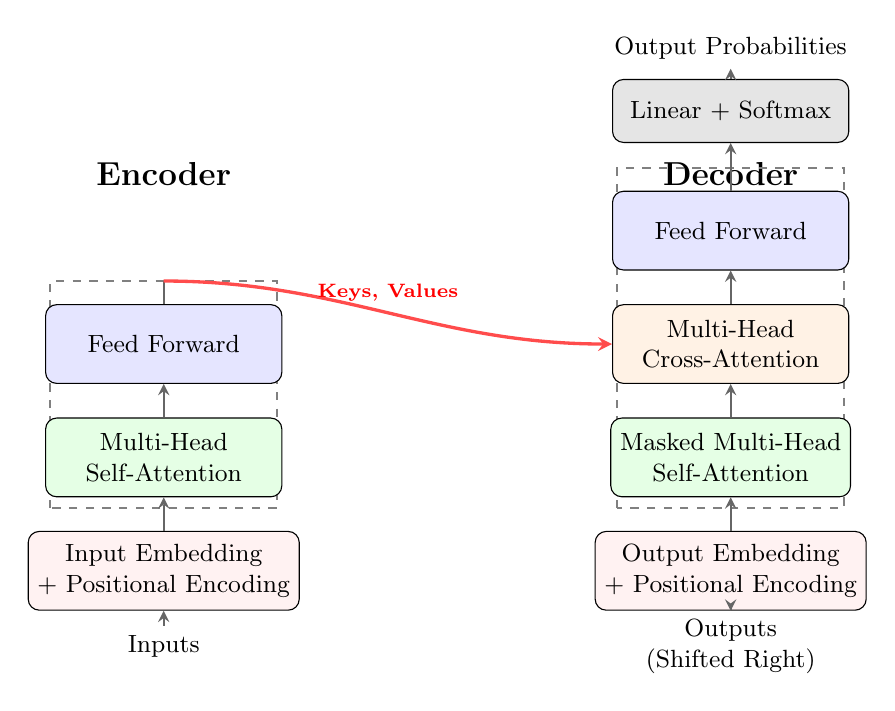
\begin{tikzpicture}[>=stealth, scale=0.8,
    % 定义通用方块样式
    block/.style={
        draw, 
        rounded corners, 
        minimum width=3cm, 
        minimum height=1cm, 
        align=center, 
        font=\small
    },
    % 定义箭头样式
    arrow/.style={->, thick, gray!80!black},
    % 修复点：定义无边框但需要换行的文本节点样式
    text_node/.style={
        align=center,
        font=\small
    }
]

    % ================== Encoder (左塔) ==================
    \begin{scope}[xshift=-4.5cm]
        \node[font=\bfseries\large] at (0, 6.5) {Encoder};
        
        % 底部输入
        \node[text_node] (enc_input) at (0, -1) {Inputs};
        \node[block, fill=pink!20] (enc_emb) at (0, 0.2) {Input Embedding\\+ Positional Encoding};
        
        % Encoder Block (用虚线框起来)
        \draw[dashed, thick, gray] (-1.8, 1.2) rectangle (1.8, 4.8);
        \node[anchor=south east, font=\scriptsize, gray] at (1.8, 1.2) {$\times N$};
        
        \node[block, fill=green!10] (enc_self) at (0, 2) {Multi-Head\\Self-Attention};
        \node[block, fill=blue!10] (enc_ffn) at (0, 3.8) {Feed Forward};
        
        % 连线
        \draw[arrow] (enc_input) -- (enc_emb);
        \draw[arrow] (enc_emb) -- (enc_self);
        \draw[arrow] (enc_self) -- (enc_ffn);
        
        % 定义一个Encoder输出点，供后面连线使用
        \coordinate (enc_out_point) at (0, 4.8); 
        \draw[thick, gray!80!black] (enc_ffn) -- (enc_out_point);
    \end{scope}

    % ================== Decoder (右塔) ==================
    \begin{scope}[xshift=4.5cm]
        \node[font=\bfseries\large] at (0, 6.5) {Decoder};
        
        % 底部输入 (【修复点】：添加 align=center)
        \node[text_node] (dec_input) at (0, -1) {Outputs\\(Shifted Right)};
        \node[block, fill=pink!20] (dec_emb) at (0, 0.2) {Output Embedding\\+ Positional Encoding};
        
        % Decoder Block (虚线框)
        \draw[dashed, thick, gray] (-1.8, 1.2) rectangle (1.8, 6.6);
        \node[anchor=south east, font=\scriptsize, gray] at (1.8, 1.2) {$\times N$};
        
        \node[block, fill=green!10] (dec_self) at (0, 2) {Masked Multi-Head\\Self-Attention};
        \node[block, fill=orange!10] (dec_cross) at (0, 3.8) {Multi-Head\\Cross-Attention};
        \node[block, fill=blue!10] (dec_ffn) at (0, 5.6) {Feed Forward};
        
        % 顶部输出
        \node[block, fill=gray!20, minimum height=0.8cm] (linear) at (0, 7.5) {Linear + Softmax};
        \node[text_node] (final_prob) at (0, 8.5) {Output Probabilities};
        
        % 连线
        \draw[arrow] (dec_input) -- (dec_emb);
        \draw[arrow] (dec_emb) -- (dec_self);
        \draw[arrow] (dec_self) -- (dec_cross);
        \draw[arrow] (dec_cross) -- (dec_ffn);
        \draw[arrow] (dec_ffn) -- (linear);
        \draw[arrow] (linear) -- (final_prob);
    \end{scope}

    % ================== 关键连接 (Cross Attention) ==================
    % 从左塔的顶部 (enc_out_point) 连到右塔的中间 (dec_cross)
    \draw[->, very thick, red!70] (enc_out_point) 
        to[out=0, in=180] node[midway, above, font=\scriptsize\bfseries, red] {Keys, Values} 
        (dec_cross.west);

\end{tikzpicture}
\caption{Transformer 架构示意图：左侧 Encoder 生成的 K、V 矩阵传递给右侧 Decoder 的每一层 Cross-Attention 模块。}
\end{figure}

\paragraph{Encoder}
Encoder的输入是源语言句子（如英语），结构是多层自注意力 + 前馈网络，输出是源句子的表示。

\paragraph{Decoder}
Decoder的输入是目标语言的已生成部分（如法语），结构是掩码自注意力 + 交叉注意力 + 前馈网络，输出是下一个词的概率分布。

% ------------------------------------------------------------------------------------
\subsection{只用Decoder：GPT的选择}
% ------------------------------------------------------------------------------------

GPT系列模型简化了结构，\textbf{只用Decoder}：

\begin{figure}[htbp]
\centering
\begin{tikzpicture}[>=stealth, scale=0.8,
    block/.style={draw, rounded corners, minimum width=3cm, minimum height=0.7cm, font=\small}]
    
    % 输入
    \node[block, fill=blue!20] (input) at (0, 0) {输入 Token};
    \node[block, fill=purple!20] (embed) at (0, 1) {嵌入 + 位置编码};
    
    % Decoder块
    \draw[thick, dashed] (-2, 1.8) rectangle (2, 5.2);
    \node[font=\scriptsize] at (0, 5) {$\times L$层};
    
    \node[block, fill=green!20] (attn) at (0, 2.5) {掩码自注意力};
    \node[block, fill=orange!20] (ff) at (0, 3.5) {前馈网络};
    \node[block, fill=gray!30] (ln) at (0, 4.5) {层归一化};
    
    % 输出
    \node[block, fill=red!20] (lm) at (0, 6) {语言模型头};
    \node[block, fill=yellow!20] (out) at (0, 7) {下一个Token概率};
    
    % 箭头
    \draw[->, thick] (input) -- (embed);
    \draw[->, thick] (embed) -- (attn);
    \draw[->, thick] (attn) -- (ff);
    \draw[->, thick] (ff) -- (ln);
    \draw[->, thick] (ln) -- (lm);
    \draw[->, thick] (lm) -- (out);
    
    % 残差连接
    \draw[->, thick, gray, dashed] (embed) -- ++(-1.5, 0) -- ++(0, 2) -- (attn);
    \draw[->, thick, gray, dashed] (attn) -- ++(1.5, 0) -- ++(0, 1) -- (ff);
    
\end{tikzpicture}
\caption{GPT的纯Decoder结构}
\end{figure}

\paragraph{掩码自注意力}

GPT是\textbf{自回归}模型：生成第 $t$ 个词时，只能看到前 $t-1$ 个词。

这通过\textbf{注意力掩码}实现：把未来位置的注意力分数设为 $-\infty$，softmax后变成0。

\begin{equation}
    \text{Mask}_{ij} = \begin{cases}
        0 & \text{if } j \leq i \\
        -\infty & \text{if } j > i
    \end{cases}
\end{equation}

\begin{figure}[htbp]
\centering
\begin{tikzpicture}[scale=0.6]
    % 掩码矩阵
    \foreach \i in {1,...,5} {
        \foreach \j in {1,...,5} {
            \ifnum\j>\i
                \fill[red!30] (\j-1, 5-\i) rectangle (\j, 6-\i);
            \else
                \fill[green!30] (\j-1, 5-\i) rectangle (\j, 6-\i);
            \fi
        }
    }
    \draw[step=1, thick] (0, 0) grid (5, 5);
    
    % 标签
    \node[left] at (0, 4.5) {$t=1$};
    \node[left] at (0, 3.5) {$t=2$};
    \node[left] at (0, 2.5) {$t=3$};
    \node[left] at (0, 1.5) {$t=4$};
    \node[left] at (0, 0.5) {$t=5$};
    
    \node[below] at (0.5, 0) {1};
    \node[below] at (1.5, 0) {2};
    \node[below] at (2.5, 0) {3};
    \node[below] at (3.5, 0) {4};
    \node[below] at (4.5, 0) {5};
    
    % 图例
    \fill[green!30] (7, 4) rectangle (8, 5);
    \node[right] at (8, 4.5) {可以看到};
    \fill[red!30] (7, 2.5) rectangle (8, 3.5);
    \node[right] at (8, 3) {被遮挡};
    
\end{tikzpicture}
\caption{因果掩码：位置 $t$ 只能看到 $1, 2, \ldots, t$ 的信息}
\end{figure}

% ------------------------------------------------------------------------------------
\subsection{一个Transformer层的完整流程}
% ------------------------------------------------------------------------------------

让我们详细追踪一个Transformer层的数据流：

\begin{enumerate}
    \item \textbf{输入}：$X \in \mathbb{R}^{T \times d}$
    
    \item \textbf{层归一化}：$X' = \text{LayerNorm}(X)$
    
    \item \textbf{计算Q、K、V}：
    \begin{align}
        Q &= X' W_Q \in \mathbb{R}^{T \times d_k} \\
        K &= X' W_K \in \mathbb{R}^{T \times d_k} \\
        V &= X' W_V \in \mathbb{R}^{T \times d_v}
    \end{align}
    
    \item \textbf{计算注意力分数}：
    \begin{equation}
        A = \text{softmax}\left(\frac{QK^\top}{\sqrt{d_k}} + \text{Mask}\right) \in \mathbb{R}^{T \times T}
    \end{equation}
    
    \item \textbf{加权求和}：$\text{Attn} = AV \in \mathbb{R}^{T \times d_v}$
    
    \item \textbf{残差连接}：$X_1 = X + \text{Attn} \cdot W_O$
    
    \item \textbf{前馈网络}：
    \begin{equation}
        X_2 = X_1 + \text{MLP}(\text{LayerNorm}(X_1))
    \end{equation}
    其中 $\text{MLP}(x) = \text{激活函数}(xW_1 + b_1)W_2 + b_2$
    
    \item \textbf{输出}：$X_2 \in \mathbb{R}^{T \times d}$
\end{enumerate}
\tryit{按这八步用 PyTorch 写一个 \texttt{TransformerBlock} 类（约 40 行），用 \texttt{torch.autograd.gradcheck} 检查；附录C“代码实现”一节给出了其中注意力部分的参考实现。}

% ====================================================================================
\section{输入输出：实际使用指南}
% ====================================================================================

理解了Transformer的结构后，让我们看看实际使用时的输入输出是怎样的。

% ------------------------------------------------------------------------------------
\subsection{输入格式}
% ------------------------------------------------------------------------------------

对于GPT类模型，输入是一个\textbf{token序列}：

\begin{center}
\begin{tabular}{ll}
\toprule
格式 & 说明 \\
\midrule
原始文本 & “What is the capital of France?” \\
Token IDs & $[2061, 318, 262, 3139, 286, 4881, 30]$ \\
嵌入向量 & $X \in \mathbb{R}^{7 \times d}$ \\
\bottomrule
\end{tabular}
\end{center}

\paragraph{特殊Token}

大多数模型使用一些特殊token：\texttt{<BOS>} 或 \texttt{<s>} 标记句子开始，\texttt{<EOS>} 或 \texttt{</s>} 标记句子结束，\texttt{<PAD>} 用于填充（让不同长度的序列对齐），\texttt{<UNK>} 表示未知词（不在词表中）。

\paragraph{批处理}

实际训练时，多个序列会被打包成一个\textbf{批次}（Batch）：

\begin{equation}
    X \in \mathbb{R}^{B \times T \times d}
\end{equation}

其中 $B$ 是批大小，$T$ 是序列长度，$d$ 是嵌入维度。

% ------------------------------------------------------------------------------------
\subsection{输出格式}
% ------------------------------------------------------------------------------------

Transformer的输出也是一个序列，每个位置对应一个向量：

\begin{equation}
    Y \in \mathbb{R}^{T \times d}
\end{equation}

\paragraph{语言模型任务}

对于生成下一个词的任务，需要把输出向量映射到词表大小的概率分布：

\begin{equation}
    P = \text{softmax}(Y W_{\text{vocab}} + b) \in \mathbb{R}^{T \times V}
\end{equation}

$P_{t,v}$ 表示在位置 $t$ 生成词 $v$ 的概率。

\paragraph{生成过程（自回归）}

生成文本时，模型一次只生成一个token，然后把新token加入输入，继续生成：

\begin{figure}[htbp]
\centering
\begin{tikzpicture}[>=stealth, scale=0.8]
    % 步骤1
    \node at (-2, 3) {\textbf{步骤1:}};
    \node[draw, rectangle, fill=blue!20] at (1, 3) {What is};
    \node at (3, 3) {$\rightarrow$};
    \node[draw, rectangle, fill=green!20] at (4.5, 3) {the};
    
    % 步骤2
    \node at (-2, 2) {\textbf{步骤2:}};
    \node[draw, rectangle, fill=blue!20] at (1.5, 2) {What is the};
    \node at (3.5, 2) {$\rightarrow$};
    \node[draw, rectangle, fill=green!20] at (5.2, 2) {capital};
    
    % 步骤3
    \node at (-2, 1) {\textbf{步骤3:}};
    \node[draw, rectangle, fill=blue!20] at (2, 1) {What is the capital};
    \node at (4.5, 1) {$\rightarrow$};
    \node[draw, rectangle, fill=green!20] at (6, 1) {of};
    
    % 继续
    \node at (3, 0) {$\vdots$};
\end{tikzpicture}
\caption{自回归生成：每次生成一个token，然后作为下一次的输入}
\end{figure}



\sidenoteplain{KV Cache是企业进行大模型部署的关键步骤，理解它对优化推理速度很重要。}
\subsection{KV Cache：为什么能大幅加速推理？}
% ------------------------------------------------------------------------------------

自回归大模型在\textbf{生成第 $t$ 个 token} 时，需要看见前面所有的 token：
\[
p(x_t \mid x_1, x_2, \dots, x_{t-1}).
\]
在 Transformer 里，这意味着第 $t$ 个位置的 Query 要和前面 $1\sim t$ 个位置的 Key/Value 做 Self-Attention。

如果\textbf{完全不做缓存}，第 $t$ 步要重新计算：
\[
K_1, V_1,\, K_2, V_2,\, \dots,\, K_t, V_t,
\]
生成长度为 $T$ 的一句话，总计算量大约是 $O(T^2)$：越到后面越慢。

\paragraph{关键观察：历史的 K/V 根本不会变}

在解码阶段，每个位置 $i$ 的
\[
K_i = W_K h_i, \quad V_i = W_V h_i
\]
一旦算出来，就\textbf{永远不会再被修改}。但我们在后续每一步里，会一遍又一遍地用到这些 K/V。

\textbf{KV Cache 的想法就很简单}：第一次看到某个 token 时，把它的 $K_i, V_i$ 算出来；以后再生成新 token 时，\textbf{不再重新算}前面的 $K_1,\dots,K_{t-1}$，直接\textbf{从缓存里读出来用}。

这样，生成每个新 token 时，只需要：
\[
\text{计算新的 } K_t, V_t,\quad \text{然后与缓存中的 } K_{1:t-1}, V_{1:t-1} \text{ 做 Attention。}
\]
复杂度从“每次重算 $1\sim t$ 个”变成“只算第 $t$ 个”：省掉的是历史 K/V 的重复投影（$O(T^2 d) \to O(T d)$）；注意力本身每步仍要算 $q_t$ 与全部历史的点积，总量仍是 $O(T^2)$。

\sidenoteplain{直观地说：本来每写一个字都要把全文再读一遍，现在改成“以前读过的都用笔记查”，当然快很多。}

\paragraph{图示理解}

\begin{figure}[H]
\centering
\begin{tikzpicture}[>=stealth, scale=0.8, font=\scriptsize]

    % 样式定义
    \tikzstyle{block_new} = [draw, fill=blue!40, minimum size=0.6cm, anchor=center]
    \tikzstyle{block_recalc} = [draw, fill=red!30, minimum size=0.6cm, anchor=center]
    \tikzstyle{block_cache} = [draw, fill=green!20, dashed, minimum size=0.6cm, anchor=center]
    
    % ================= 左侧：无缓存 (Standard Attention) =================
    \begin{scope}[xshift=-4.5cm]
        \node[font=\bfseries\small] at (1.5, 4.5) {无缓存：计算量爆炸};
        \node[gray] at (1.5, 4) {(每次都要重算历史)};
        
        % 时间步 t=1
        \node[left] at (-0.5, 3) {$t=1$};
        \node[block_new] at (0, 3) {1};
        
        % 时间步 t=2
        \node[left] at (-0.5, 2) {$t=2$};
        \node[block_recalc] at (0, 2) {1}; % 重算
        \node[block_new] at (0.7, 2) {2};
        
        % 时间步 t=3
        \node[left] at (-0.5, 1) {$t=3$};
        \node[block_recalc] at (0, 1) {1}; % 重算
        \node[block_recalc] at (0.7, 1) {2}; % 重算
        \node[block_new] at (1.4, 1) {3};
        
        % 时间步 t=4
        \node[left] at (-0.5, 0) {$t=4$};
        \node[block_recalc] at (0, 0) {1}; % 重算
        \node[block_recalc] at (0.7, 0) {2}; % 重算
        \node[block_recalc] at (1.4, 0) {3}; % 重算
        \node[block_new] at (2.1, 0) {4};
        
        % 标注浪费
        \draw[<-, thick, red] (0.35, 0.5) -- (1.5, 1.5) node[right, red, align=left] {红色块都是\\重复计算！};
    \end{scope}
    
    % 分隔线
    \draw[dashed, gray] (0, -0.5) -- (0, 4.5);

    % ================= 右侧：KV Cache =================
    \begin{scope}[xshift=2cm]
        \node[font=\bfseries\small] at (1.5, 4.5) {KV Cache：增量计算};
        \node[gray] at (1.5, 4) {(空间换时间)};
        
        % 时间步 t=1
        \node[block_new] at (0, 3) {1};
        \node[right, gray, scale=0.8] at (0.4, 3) {存入Cache};
        
        % 时间步 t=2
        \node[block_cache] at (0, 2) {1}; % 缓存
        \node[block_new] at (0.7, 2) {2};
        
        % 时间步 t=3
        \node[block_cache] at (0, 1) {1};
        \node[block_cache] at (0.7, 1) {2};
        \node[block_new] at (1.4, 1) {3};
        
        % 时间步 t=4
        \node[block_cache] at (0, 0) {1};
        \node[block_cache] at (0.7, 0) {2};
        \node[block_cache] at (1.4, 0) {3};
        \node[block_new] at (2.1, 0) {4};
        
        % 标注
        \draw[decorate, decoration={brace, amplitude=5pt}, green!50!black] (0-0.3, -0.4) -- (1.4+0.3, -0.4);
        \node[below, green!50!black] at (0.7, -0.6) {直接读取，不计算};
        
        \draw[->, blue, thick] (2.1, -0.4) -- (2.1, -0.6) node[below] {只算这个};
    \end{scope}

\end{tikzpicture}
\caption{KV Cache 原理对比：左图展示了标准的 Attention 机制在解码时存在大量冗余计算（红色部分）；右图展示了 KV Cache 如何通过复用历史计算结果（绿色虚线框）将计算复杂度从 $O(T^2)$ 降低为 $O(T)$。}
\end{figure}

\paragraph{为什么只缓存 K/V，不缓存 Q？}

对于第 $t$ 个位置：

\[
\text{Attention}(q_t,\; K_{1:t},\; V_{1:t}).
\]

$q_t$ 只依赖当前这个 token（以及当前位置），\textbf{每次都不一样}，不能提前算，也没必要缓存；而 $K_{1:t-1}, V_{1:t-1}$ 来自历史 token，\textbf{一旦算完就不再改变}，非常适合缓存。因此只缓存 K 和 V 就足够了，这也是名词叫 \emph{KV Cache} 的原因。

% -------------------------------------------------------
\paragraph{KV Cache 的显存开销从哪里来？}

缓存不是免费的，它会占用显存。典型估算公式为：
\begin{equation}
    \text{显存} 
    \;\approx\; 
    2 \times L \times T \times d \times \text{batch\_size} \times \text{precision},
\end{equation}
其中：

\begin{itemize}
    \item 因子 $2$：一份是 Key，一份是 Value；
    \item $L$：Transformer 的层数（每一层都有自己的 K/V，需要各存一份）；
    \item $T$：序列长度（越长，对应的缓存就越大）；
    \item $d$：每个位置向量的维度（hidden size，例如 4096）；
    \item $\text{batch\_size}$：一次同时生成多少条序列；
    \item $\text{precision}$：每个数占多少字节（FP16 是 2 字节，FP32 是 4 字节）。
\end{itemize}

\begin{example}[一个简单的数量级估算]
假设：
\begin{gather*}
L = 32,\quad
T = 2048,\quad
d = 4096,\\
\text{batch\_size}=1,\quad
\text{precision} = 2\ \text{bytes (FP16)}.
\end{gather*}
则 KV Cache 需要的显存大约为
\[
2 \times 32 \times 2048 \times 4096 \times 2
\;\approx\; 1.07\times 10^9\ \text{bytes} \;\approx\; 1\ \text{GB}.
\]
这只是\textbf{缓存}占掉的显存，还不包括模型参数本身！
\end{example}

这也是为什么上下文越长（$T$ 越大），显存越吃紧；工程上要对 KV Cache 做\textbf{量化}（比如用 \texttt{int8}、\texttt{int4} 存储）来减小显存开销；企业部署大模型时，KV Cache 是\textbf{必须精细优化}的一环。
\preview{附录C会把这个公式扩展成完整的显存预算表：权重、梯度、优化器状态、激活值、KV Cache，并讨论“显存的影子价格”。}




% ------------------------------------------------------------------------------------
\subsection{上下文长度限制}
% ------------------------------------------------------------------------------------

Transformer有一个重要限制：\textbf{最大上下文长度}。GPT-3是2048 tokens，GPT-4是8192 / 32768 tokens，Claude则达到100K+ tokens。

\paragraph{为什么有长度限制？}

原因有三：注意力复杂度是 $O(T^2)$，长序列计算量巨大；某些位置编码方式限制了最大长度；KV Cache随长度线性增长，受显存限制。

\paragraph{超长文本怎么办？}

常见做法有三种：分块处理，把长文档切成多个块，分别处理；滑动窗口，只保留最近的 $T$ 个token；长度外推，用特殊的位置编码支持更长序列。

% ====================================================================================
% 代码演示结果
\begin{figure}[htbp]
\centering
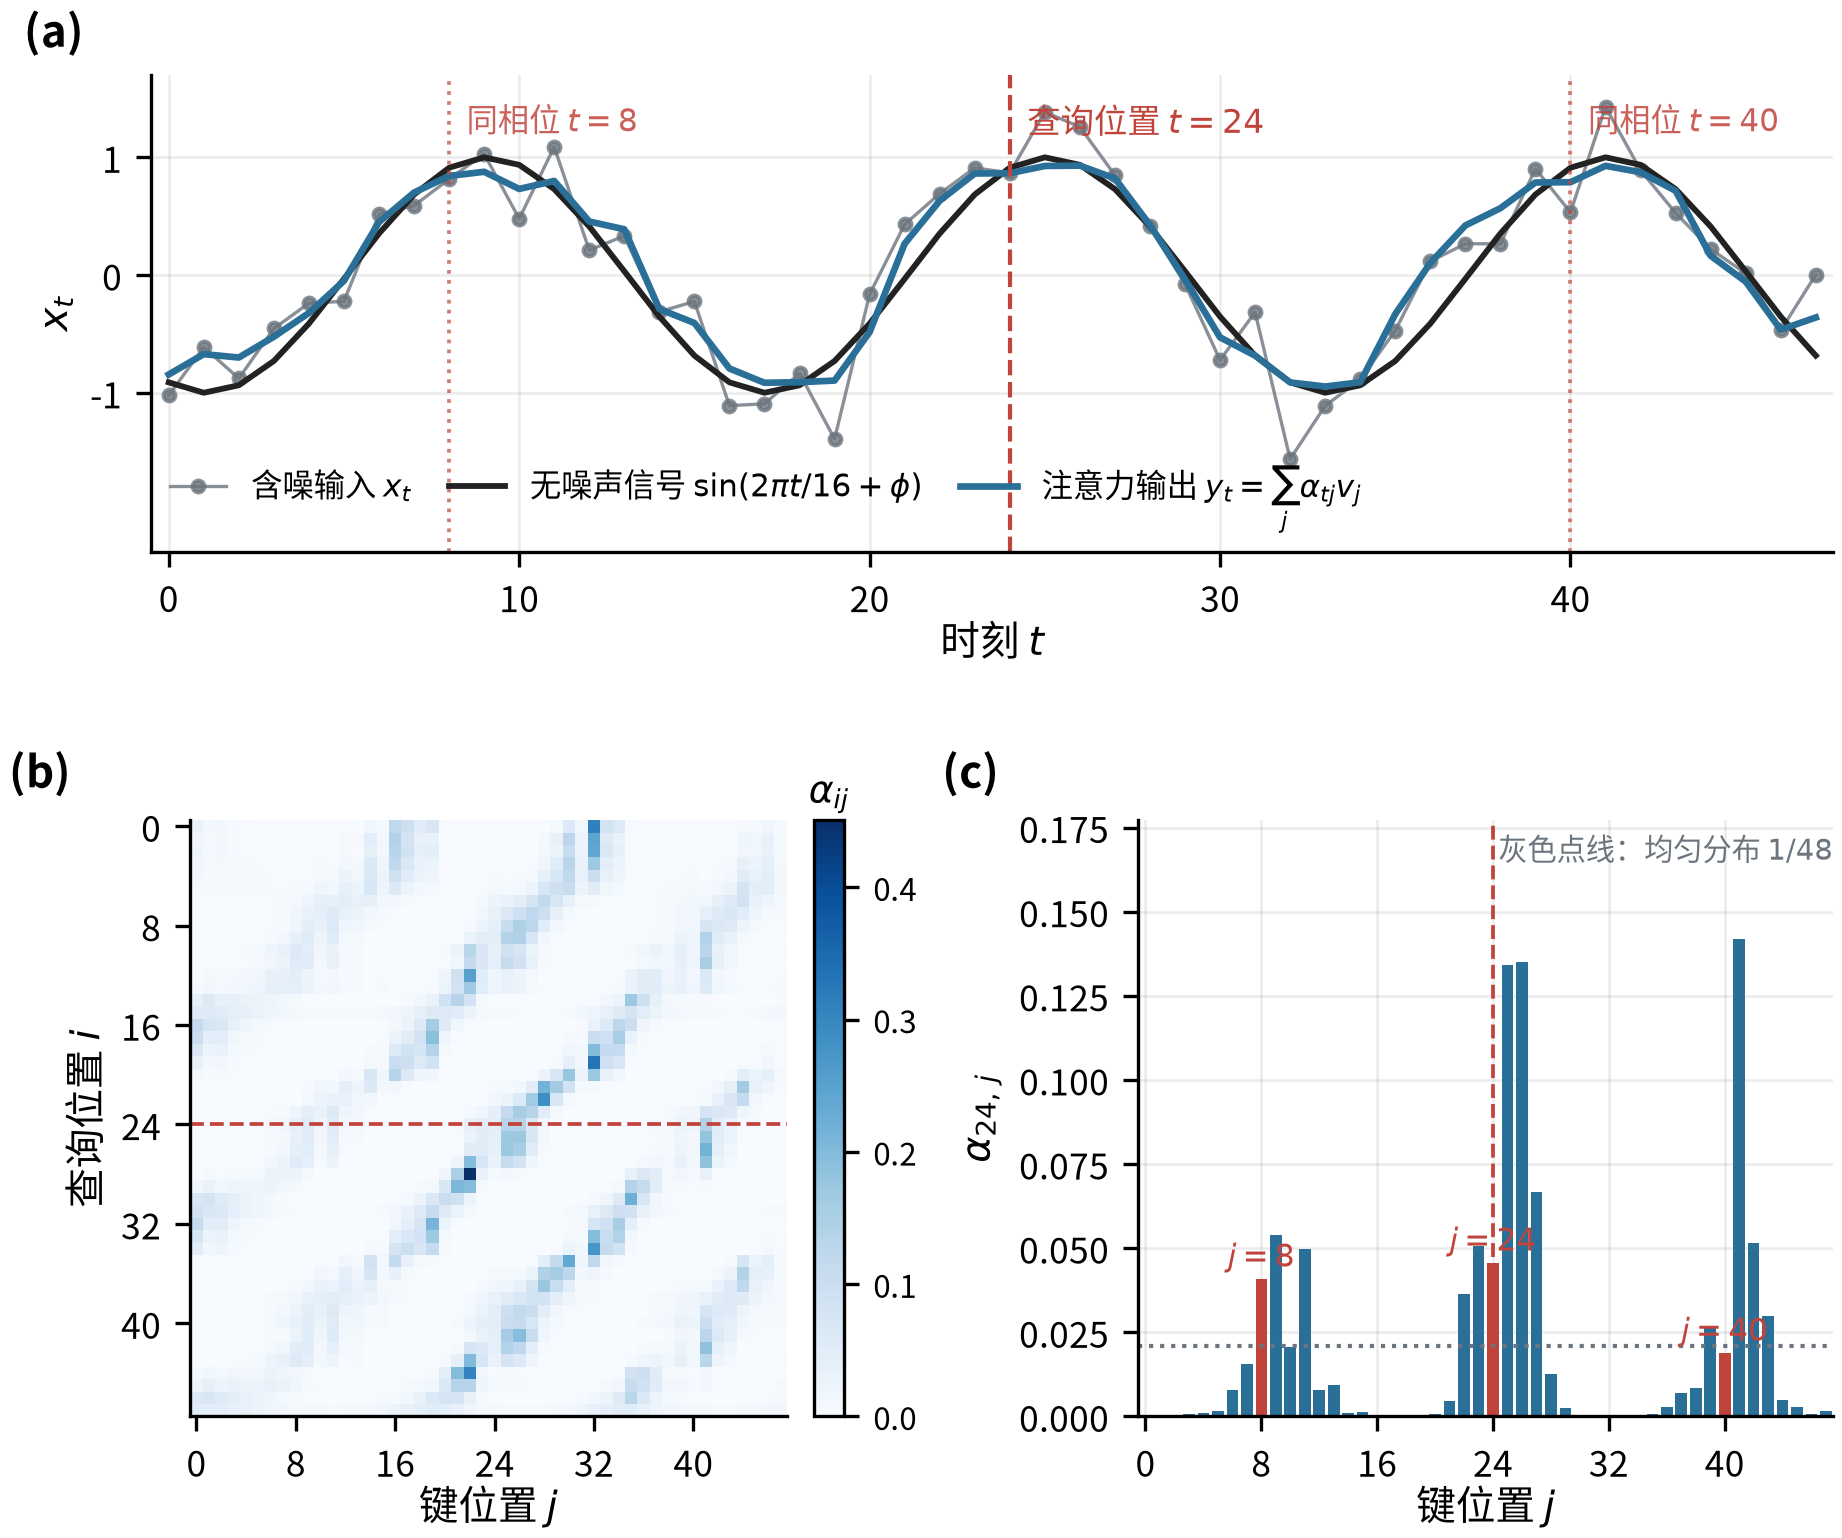
\includegraphics[width=0.98\textwidth]{figs_chap11/chap11_fig1.png}
\caption{一个真实训练出来的单头自注意力（\texttt{code\_chap11/chap11\_figures.py}）：输入是含噪的正弦序列 $x_t=\sin(2\pi t/16+\phi)+\varepsilon_t$（$T=48$，三个周期），$Q,K,V$ 由最近 4 个采样值线性映射得到，训练目标是还原无噪声的信号。（a）含噪输入（灰点）、真实信号（黑线）与注意力输出（蓝线）：输出的均方误差约为输入噪声的一半。（b）注意力矩阵 $\alpha_{ij}=\mathrm{softmax}_j(q_i\cdot k_j/\sqrt{d_k})$：平行于对角线、间距为 16 的条纹说明模型学会了``关注相位相同的时刻''。（c）查询位置 $t=24$ 的注意力分布：权重集中在 $j\approx 8,24,40$ 三簇（合计约 0.95），其余位置几乎为零——注意力就是按相似度加权的平均，即正文所说的 softmax 核回归。}
\label{fig:chap11_attention}
\end{figure}

\begin{figure}[htbp]
\centering
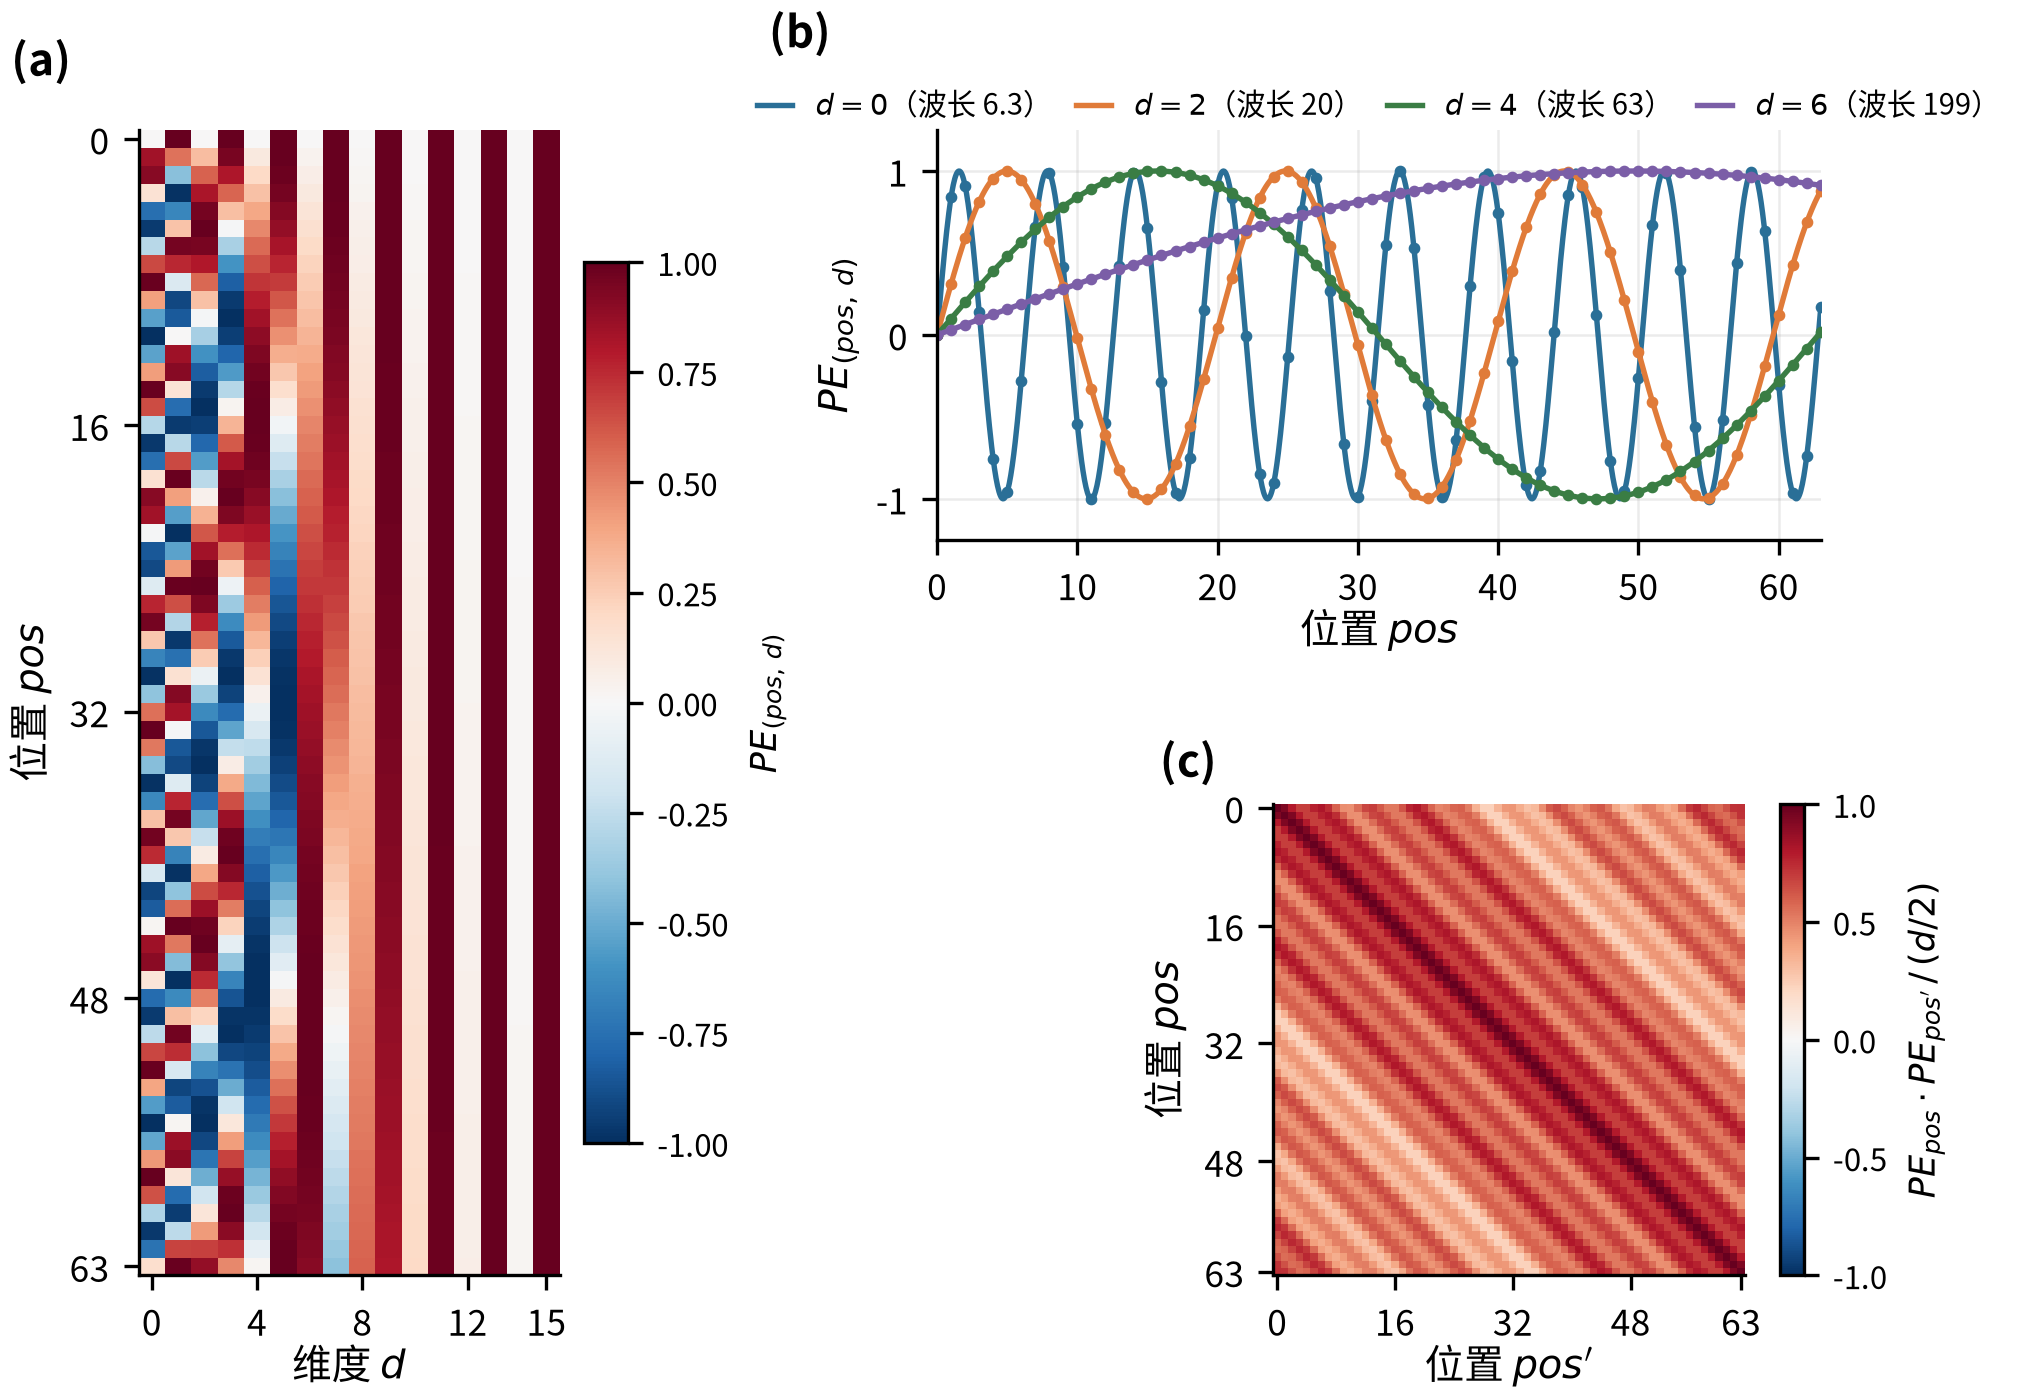
\includegraphics[width=0.95\textwidth]{figs_chap11/chap11_fig2.png}
\caption{正弦位置编码（$d_{\text{model}}=16$，位置 $0\sim 63$）。（a）编码矩阵 $PE_{(pos,d)}$：低维度变化快（高频），高维度变化慢（低频），最右几列在 64 个位置内几乎不变。（b）维度 $0,2,4,6$ 的正弦分量，波长分别为 $6.3,20,63,199$：一个位置的编码就是一组不同频率的``时钟指针''。（c）位置之间的归一化点积 $PE_{pos}\cdot PE_{pos'}/(d/2)$：矩阵沿对角线平移不变，只依赖相对位置 $pos-pos'$，相邻位置最相似——这正是``$PE_{pos+k}$ 是 $PE_{pos}$ 的线性变换''的体现。}
\label{fig:chap11_positional_encoding}
\end{figure}


% ====================================================================================
\section{视觉--语言模型：把图像也变成 token}
% ====================================================================================

到目前为止，本章的 Transformer 只吃一种东西：文本 token。可是物理智能要面对的世界不是一串字，而是一张张图像、一段段视频。让语言模型“睁开眼睛”的办法，出人意料地简单：\textbf{不改 Transformer，改输入}——把图像也变成一串 token，和文本 token 拼在同一条序列里，剩下的交给注意力。本节沿着这条思路走一遍：图像怎么切成 token，视觉编码器怎么训，怎么接到语言模型上，以及整套系统按什么配方训练。每一步我们照例问同样的三个问题：目标是什么、约束是什么、$\lambda$ 代表什么。

% ------------------------------------------------------------------------------------
\subsection{为什么要把图像变成 token}
% ------------------------------------------------------------------------------------

回顾本章“注意力机制”一节：注意力只做一件事——对一组向量按相似度做加权平均。它不关心这些向量从哪里来，是一个词、一个像素块，还是一段声音。这意味着 Transformer 天然是一个\textbf{与模态无关}的机器：只要你能把任何信号表示成“一串 $d$ 维向量”，它就能处理。

\begin{keyidea}[感知的统一接口]
Transformer 只认一种输入：形状为 $T \times d$ 的向量序列。因此，让模型“看见”的问题，就被转化为一个\textbf{接口问题}：
\begin{equation}
    \text{图像} \;\xrightarrow{\;\text{某种编码器}\;}\; X_{\text{img}} \in \mathbb{R}^{N \times d}, \qquad
    \text{文本} \;\xrightarrow{\;\text{分词 + 嵌入}\;}\; X_{\text{txt}} \in \mathbb{R}^{T \times d},
\end{equation}
然后把两者拼成一条长度为 $N + T$ 的序列送进同一个 Transformer。文本、图像、音频、机器人的关节角度，在这个接口之后都是一样的东西——token。
\end{keyidea}

这个想法之所以重要，是因为它把“多模态”从一个架构问题变成了一个\textbf{表示问题}：我们不需要为每种感官设计一套新的网络，只需要为每种感官设计一个“翻译成 token”的前端。

% ------------------------------------------------------------------------------------
\subsection{ViT：把图片切成 patch}
% ------------------------------------------------------------------------------------

一张 $224 \times 224$ 的彩色图像有 $224 \times 224 \times 3 \approx 150{,}000$ 个数。如果把每个像素当一个 token，序列长度 $T = 50{,}176$，注意力的 $O(T^2)$ 代价会立刻把我们压垮。视觉 Transformer（Vision Transformer, ViT，2020）的解法是：不看像素，看\textbf{小块}（patch）。
\storynote{Alexey Dosovitskiy}{2020 年，Google 的 Dosovitskiy 等人发表《An Image Is Worth 16x16 Words》。标题就是全部思想：一张图等于 196 个“单词”。当时很多人认为卷积的归纳偏置不可替代，而这篇论文表明，只要数据够多，一个几乎没改动的文本 Transformer 也能在图像分类上追平甚至超过卷积网络。}

\paragraph{patch 化}

把图像切成互不重叠的 $P \times P$ 小块。对 $224 \times 224$ 的图，取 $P = 16$ 时每边 $224/16 = 14$ 块，共 $14^2 = 196$ 个 patch；取 $P = 14$ 时每边 $224/14 = 16$ 块，共 $16^2 = 256$ 个 patch。每个 patch 展平后是一个 $P^2 \cdot 3$ 维的向量（$P = 16$ 时是 768 维）。于是一张图从“$150{,}000$ 个像素”变成了“196 个 768 维向量”——序列长度降到了和一段文本差不多的量级。

\paragraph{线性嵌入与位置编码}

接下来的步骤和本章“文本到数字”一节完全平行：
\begin{equation}
    z_i = W_{\text{patch}}\, \mathrm{vec}(\text{patch}_i) + p_i, \qquad i = 1, \dots, N,
\end{equation}
其中 $W_{\text{patch}} \in \mathbb{R}^{d \times 3P^2}$ 是一个线性层（相当于文本的“查词表”，只不过这里是乘一个矩阵而不是查一行），$p_i$ 是位置编码。位置编码在这里更加不可或缺：注意力本身不知道两个 patch 谁在左谁在右、谁在上谁在下，把 196 个 patch 打乱顺序它也看不出来。ViT 用的是可学习的位置编码，把二维网格按行展开成一维序号即可；也有工作显式地用二维坐标构造编码。

\paragraph{汇聚：[CLS] 还是均值}

经过 $L$ 层 Transformer 后，我们得到 $N$ 个输出向量。如果任务需要“整张图的一个向量”（例如分类或者和一句话做对比），有两种常见做法：在序列前面多加一个可学习的特殊 token \texttt{[CLS]}，让它通过注意力从所有 patch 里“收集”信息，取它的输出；或者干脆对 $N$ 个输出向量取平均（均值池化）。两者效果通常相近。

\paragraph{和文本 token 的三点不同}

第一是\textbf{连续与离散}之别：文本 token 是词表里的整数 ID，图像 patch 是连续向量。这意味着图像 token 没有“词表”，也就没法像文本那样用 softmax 交叉熵去“预测下一个 patch”——这一点在后面讨论训练损失时会再回来。第二是\textbf{序列长度}：一句话通常几十个 token，而一张 $224 \times 224$ 的图是 196 或 256 个；分辨率翻倍，patch 数翻四倍。图像是“话多”的模态。第三是\textbf{信息密度}：一个词几乎每个都有意义，而相邻的 patch 高度冗余（一片蓝天切出的几十个 patch 几乎一样）。这为后面的“压缩”留下了空间。

% ------------------------------------------------------------------------------------
\subsection{视觉编码器怎么训：对比学习}
% ------------------------------------------------------------------------------------

ViT 只是一个架构，它输出的向量有没有“意义”，取决于用什么目标去训它。最早的 ViT 用图像分类标签训练——这条路线的数据基础是李飞飞团队 2009 年发布的 ImageNet，它的标注是靠亚马逊 Mechanical Turk 众包完成的。而今天视觉--语言模型里的视觉编码器，几乎都用\textbf{图文对比学习}（contrastive learning）训练，代表是 CLIP（2021）和 SigLIP（2023）。

想法很直接：互联网上有海量“图片 + 文字说明”的配对——Radford 等人 2021 年发布的 CLIP 就用了 4 亿对。我们训练一个图像编码器 $f$ 和一个文本编码器 $g$，让配对的图和文在同一个向量空间里靠近，不配对的远离。取一个批次的 $B$ 个图文对，把编码后的向量归一化到单位球面上：$u_i = f(\text{img}_i)/\|f(\text{img}_i)\|$，$v_j = g(\text{txt}_j)/\|g(\text{txt}_j)\|$，相似度就是内积 $s_{ij} = u_i^\top v_j \in [-1, 1]$。

\begin{keyformula}[title=CLIP 的对比损失]
对第 $i$ 张图，在 $B$ 段文本里“选出”它的配文，这是一个 $B$ 类分类问题：
\begin{equation}
    p_{ij} = \frac{\exp(s_{ij}/\tau)}{\sum_{k=1}^{B} \exp(s_{ik}/\tau)}, \qquad
    \ell_{\text{img}\to\text{txt}} = -\frac{1}{B}\sum_{i=1}^{B} \log p_{ii}.
    \label{eq:clip_loss}
\end{equation}
对称地再做一遍“文找图”，两者取平均就是 CLIP 的损失。$\tau$ 是温度。把 $-\log p_{ii}$ 展开，每一项都可以拆成两部分：
\begin{equation}
    -\log p_{ii} = -\frac{s_{ii}}{\tau} + \log \sum_{k=1}^{B} e^{s_{ik}/\tau}.
    \label{eq:clip_split}
\end{equation}
\end{keyformula}

式~\eqref{eq:clip_split} 的拆分值得多看一眼：第一项把匹配对的相似度\textbf{往上拉}，第二项是配分函数的对数，把所有对的相似度\textbf{往下压}。这正是第4章的结构——$p_{ij}$ 是一个玻尔兹曼分布，$\log\sum_k e^{s_{ik}/\tau}$ 就是 $\log Z$。
\review{第4章}{在给定“期望相似度”约束下最大化熵，解是 $p_{ij} \propto \exp(\beta s_{ij})$，$\beta$ 是这条约束的拉格朗日乘子。对比学习里的 $1/\tau$ 就是这个 $\beta$：温度是乘子的倒数。这和本章注意力里的 $1/\sqrt{d_k}$ 是同一个角色。}

\begin{keyidea}[对比学习的目标 / 约束 / $\lambda$]
\textbf{目标}是最大化匹配对的对数似然 $\sum_i \log p_{ii}$，等价于让 $u_i$ 和 $v_i$ 的内积在所有候选中脱颖而出。\textbf{约束}有两条。第一条是 $u_i, v_j$ 落在单位球面上，$\|u_i\| = \|v_j\| = 1$：没有它，模型只要把向量的模长放大就能让 $\log Z$ 项随意变化，“相似”就失去了意义；归一化是这条约束的硬性实现。第二条是每张图对 $B$ 段文本的“注意力” $p_{i\cdot}$ 必须是一个概率分布——归一化约束，它的乘子给出 $\log Z$，也就是式~\eqref{eq:clip_split} 的第二项。而 \textbf{$\lambda$} 就是 $1/\tau$，即“期望相似度”约束的乘子：$\tau$ 越小，分布越尖，模型越“确信”；$\tau$ 越大，分布越平，匹配与不匹配的差别被抹平。CLIP 干脆把 $\tau$ 也设成可学习参数（初始值 $0.07$）——让模型自己决定这条约束的价格。
\end{keyidea}

SigLIP 做了一个小而重要的改动：不再要求 $p_{i\cdot}$ 在整个批次上归一化，而是对每一对 $(i, j)$ 独立地做一个二分类——“这一对是不是配对的”——用 sigmoid 损失。这去掉了上面的第二条约束，于是不再需要全批次的 $\log Z$，损失可以按对拆开计算，对 batch 大小的依赖也小得多。在本书的语言里，这是把一条全局归一化约束换成了 $B^2$ 条相互独立的局部约束。

训练好之后，我们只保留图像编码器 $f$（通常连 \texttt{[CLS]} 之前的 $N$ 个 patch 输出一起保留），它的输出向量已经“知道”哪些视觉特征对应哪些词——这是把它接到语言模型上的最好起点。

% ------------------------------------------------------------------------------------
\subsection{接到语言模型上：连接器与多模态序列}
% ------------------------------------------------------------------------------------

\begin{figure}[htbp]
\centering
\begin{tikzpicture}[>=stealth, scale=0.88, every node/.style={transform shape},
    block/.style={draw, rounded corners, minimum width=2.5cm, minimum height=0.95cm, align=center, font=\small}]
    % 第一行：图像通路
    \node[block, fill=blue!20] (img) at (0, 2.4) {图像\\$H \times W \times 3$};
    \node[block, fill=blue!20] (patch) at (3.4, 2.4) {切成 patch\\$N$ 个 $P \times P$ 小块};
    \node[block, fill=green!20] (vit) at (6.8, 2.4) {视觉编码器\\(ViT)};
    \node[block, fill=orange!20] (conn) at (10.2, 2.4) {连接器\\投影 / 重采样};
    % 第二行：文本通路与拼接
    \node[block, fill=blue!20] (txt) at (0, 0) {文本提示\\``图里是什么''};
    \node[block, fill=green!20] (emb) at (3.4, 0) {分词 + 嵌入\\$T$ 个文本 token};
    \node[block, fill=purple!20] (cat) at (6.8, 0) {拼接成一条序列\\$N' + T$ 个 token};
    % 第三行：语言模型与输出
    \node[block, fill=red!20] (llm) at (6.8, -2.4) {语言模型\\(Transformer 解码器)};
    \node[block, fill=green!20] (out) at (10.2, -2.4) {输出文本\\逐 token 生成};
    % 箭头
    \draw[->, thick] (img) -- (patch);
    \draw[->, thick] (patch) -- (vit);
    \draw[->, thick] (vit) -- node[above, font=\scriptsize] {$N$ 个向量} (conn);
    \draw[->, thick] (conn.south) |- node[pos=0.75, above, font=\scriptsize] {$N'$ 个视觉 token} (cat.east);
    \draw[->, thick] (txt) -- (emb);
    \draw[->, thick] (emb) -- (cat);
    \draw[->, thick] (cat) -- (llm);
    \draw[->, thick] (llm) -- (out);
    % 标注
    \node[below, font=\scriptsize, gray, align=center] at (3.4, -2.4) {损失只算输出文本的\\下一词预测};
\end{tikzpicture}
\caption{视觉--语言模型的数据流：图像切成 patch，经视觉编码器得到 $N$ 个向量，再由连接器变成 $N'$ 个和文本嵌入同维度的视觉 token（$N' \le N$），与文本 token 拼成一条序列送进语言模型。语言模型本身不需要为图像做任何改动。}
\label{fig:vlm_pipeline}
\end{figure}

视觉编码器输出的向量维度（例如 1024）一般和语言模型的嵌入维度（例如 4096）不一样，“语义坐标系”也不一样。中间需要一个\textbf{连接器}（connector），把视觉向量翻译成语言模型能读的 token。连接器有两种主流设计。

\paragraph{投影层：一个 patch 一个 token}

最简单的做法是一个线性层或两层 MLP：
\begin{equation}
    X_{\text{img}} = \mathrm{MLP}(Z_{\text{ViT}}) \in \mathbb{R}^{N \times d_{\text{LLM}}}.
\end{equation}
LLaVA（2023）就是这么做的：CLIP 的 ViT-L/14 编码器，接一个投影层，直接把每个 patch 变成一个 token。在 $336 \times 336$ 分辨率、$P = 14$ 下，一张图就是 $24^2 = 576$ 个 token。它的优点是不丢信息、不引入新的注意力模块；缺点是 token 多。

\paragraph{重采样：把几百个压成几十个}

另一种做法利用前面提到的冗余：用 $K$ 个\textbf{可学习的查询向量}（$K$ 远小于 $N$）对 $N$ 个 patch 做交叉注意力，把信息“吸”进 $K$ 个 token 里。Flamingo（2022）的 Perceiver Resampler 用 64 个查询，BLIP-2（2023）的 Q-Former 用 32 个。这正是本章注意力的另一种用法：查询 $Q$ 不再来自输入本身，而是一组学出来的“提问”，$K, V$ 来自 patch。序列从几百压到几十，代价是压缩必然有损，细小的文字、远处的物体可能被“平均掉”。

也有人干脆跳过视觉编码器，把 patch 线性投影后直接喂进语言模型（Fuyu，2023）。这把“感知的统一接口”贯彻到了极致，代价是语言模型必须从零学会看图，需要多得多的图像数据。

\paragraph{图文交错序列}

连接器输出的视觉 token 和文本 token 处于同一个空间，于是可以像文字一样自由排布：
\begin{center}
\texttt{<image>}$\;\underbrace{x_1 \cdots x_{N'}}_{\text{视觉 token}}\;$\texttt{</image>} 这张图里有几只猫？\texttt{<assistant>} 两只。
\end{center}
一段对话里可以有多张图、图和文交替出现，模型统统当成一条序列来处理。图像的“位置”就是它在序列中的位置——位置编码对视觉 token 照常生效。

\paragraph{注意力掩码：文本因果，图像双向}

本章“只用 Decoder”一节里，GPT 用因果掩码禁止每个 token 看到未来。对视觉 token，这个限制没有道理：一张图的左上角 patch 完全可以“看”右下角，图像内部没有先后。PaliGemma（2024）采用的 \textbf{prefix-LM} 掩码把这一点写得很清楚：把图像 token 和用户提示当作“前缀”，前缀内部\textbf{双向}注意力，只有模型要生成的“后缀”才用因果掩码。用 $\mathcal{P}$ 记前缀的位置集合，掩码可以写成
\begin{equation}
    M_{ij} =
    \begin{cases}
        1, & j \le i \quad \text{（因果：可以看过去）} \\
        1, & i \in \mathcal{P} \text{ 且 } j \in \mathcal{P} \quad \text{（前缀内部：可以互看）} \\
        0, & \text{其他}
    \end{cases}
\end{equation}
$M_{ij} = 0$ 的位置在 softmax 之前被置为 $-\infty$。这个掩码和本章 Encoder-Decoder 结构的精神一致：前缀相当于一个“编码器”，只不过它和解码器共用同一套参数。

\paragraph{高分辨率的代价：token 数暴涨}

$224 \times 224$ 看不清发票上的小字。提高分辨率最直接的办法是\textbf{切块}：把一张大图切成若干个 $336 \times 336$ 的子块，每块单独过一遍编码器，再加上一张缩小的全局缩略图。四个子块加一张缩略图，就是 $5 \times 576 = 2{,}880$ 个 token——一张图的 token 数已经超过一篇短文。视频更甚：每秒抽几帧，每帧几百个 token，一分钟视频轻松上万。
\preview{视觉 token 直接进入 KV Cache：每层每个 token 都要存一份 $K$ 和 $V$。一张高分辨率图的 2{,}880 个 token 占的显存，和 2{,}880 个文字 token 一模一样。附录C会给出可以直接套用的估算公式，并讨论显存作为一条硬约束时，它的影子价格如何决定“该不该压缩视觉 token”。}

这就是为什么“重采样压缩”和“按需分辨率”成了工程上的核心问题：视觉 token 不是免费的，它们和文本 token 一样要占 $O(T^2)$ 的注意力算力与线性增长的 KV Cache。

% ------------------------------------------------------------------------------------
\subsection{和 LLM 一起训练的三阶段配方}
% ------------------------------------------------------------------------------------

现在三个部件齐了：预训练好的视觉编码器、随机初始化的连接器、预训练好的语言模型。怎么把它们训成一个整体？当前主流配方分三个阶段。

\paragraph{阶段一：对齐预训练}

冻结视觉编码器和语言模型，\textbf{只训连接器}。数据是大量简单的图文对（一张图、一句描述），任务是“看图写说明”。这一阶段的目的很单纯：让连接器学会把视觉向量翻译成语言模型“听得懂”的 token。

\paragraph{阶段二：指令微调}

解冻语言模型（有些配方也解冻视觉编码器，但用小得多的学习率），在高质量的多模态指令数据上训练：看图问答、看图推理、多轮对话、读图表、识别文档。同时\textbf{混入一定比例的纯文本指令数据}。这一阶段模型才真正学会“按要求看图做事”。

\paragraph{阶段三：偏好对齐}

和纯文本大模型一样，最后用人类偏好数据做强化学习或直接偏好优化，重点压制多模态特有的问题——例如“幻觉”：描述图里根本不存在的物体。本书不展开这一阶段，其原理见第9章。

\paragraph{损失函数：只算文本}

三个阶段用的都是本章的下一词预测损失，但有一个关键细节：\textbf{图像 token 不预测}。设序列为 $x_1, \dots, x_{N'+T}$，用掩码 $m_t \in \{0, 1\}$ 标出需要预测的位置（只有模型应当生成的文本 token 为 1），
\begin{equation}
    \ell(\theta) = -\sum_{t} m_t \log p_\theta(x_t \mid x_{<t}).
\end{equation}
原因有两个：一是视觉 token 是连续向量，没有词表可供分类；二是在 prefix-LM 掩码下前缀内部可以互看，“预测”前缀里的 token 等于作弊。图像在这里只是\textbf{条件}，不是\textbf{目标}。
\clarify{“冻结”一个模块的意思是不更新它的参数，而\textbf{不是}不经过它反向传播。阶段一里语言模型虽然被冻结，伴随变量 $\lambda$（第8章的误差信号）仍然要从损失出发穿过整个语言模型，才能到达连接器。冻结省的是优化器状态和参数更新，不省反向传播的算力。}

\paragraph{为什么要分阶段？为什么要混纯文本？}

用本书的框架来看，这两条经验都不是“技巧”，而是一条约束的两种处理方式。

\begin{keyidea}[多模态训练的目标 / 约束 / $\lambda$]
\textbf{目标}是多模态数据上的下一词预测损失 $\ell_{\text{mm}}(\theta)$——学会看图。\textbf{约束}是语言模型原有的语言能力不能退化，写成不等式就是 $\ell_{\text{txt}}(\theta) \le \ell_{\text{txt}}(\theta_0) + \epsilon$，其中 $\theta_0$ 是预训练语言模型的参数，$\ell_{\text{txt}}$ 是纯文本数据上的损失；或者写成 $\mathrm{KL}\big(p_\theta \,\|\, p_{\theta_0}\big) \le \epsilon$。于是\textbf{拉格朗日函数}为
\begin{equation}
    \mathcal{L}(\theta, \lambda) = \ell_{\text{mm}}(\theta) + \lambda \big[\ell_{\text{txt}}(\theta) - \ell_{\text{txt}}(\theta_0) - \epsilon\big].
\end{equation}
这里的 \textbf{$\lambda$} 就是训练数据里\textbf{纯文本数据的混合比例}（或 KL 正则项的系数）。它是“不遗忘”这条约束的影子价格：把语言能力的门槛 $\epsilon$ 放松一点，多模态损失能降多少。
\end{keyidea}

有了这个视角，三阶段配方就顺理成章了。\textbf{阶段一是把约束当硬约束}：$\theta_{\text{LLM}} \equiv \theta_0$，语言能力\textbf{不可能}退化。此时连接器是随机初始化的，它送进语言模型的是一堆噪声；如果这时就放开语言模型的参数，梯度会为了“迁就噪声”把语言能力冲垮——这条约束的影子价格在此刻极高，硬约束是最便宜的处理方式。

\textbf{阶段二把硬约束换成软约束}：连接器对齐之后，视觉 token 已经“像话”了，进一步提升需要语言模型本身配合，约束的影子价格降下来，于是可以解冻。混入纯文本数据就是显式地把 $\lambda\,\ell_{\text{txt}}$ 这一项加进损失；给编码器一个更小的学习率，则是对“不要偏离 $\theta_0$”这条约束的另一种软化——每一步只允许在原参数附近的一个小邻域里移动。

\textbf{混合比例不是拍脑袋定的}：按第1章互补松弛的读法，$\lambda$ 应当由约束是否被激活来决定。实际操作中人们会监控纯文本基准的分数：分数掉了，说明约束被违反，就该调高纯文本比例——这正是“按影子价格调乘子”的手工版本。

\begin{physicalmeaning}[title=$\lambda$ 在视觉--语言模型里的两种身份]
本节出现了两个 $\lambda$，它们在同一个框架里扮演不同角色。对比学习里的 $1/\tau$ 是一个“分布层面”的乘子，决定图文匹配分布的尖锐程度，与第4章的逆温度、本章注意力的 $1/\sqrt{d_k}$ 同源；它对应的约束是“期望相似度”，是关于\textbf{单个样本内部}的约束。训练配方里的混合比例则是一个“参数层面”的乘子，决定新能力（看图）与旧能力（说话）之间的交换率；它对应的约束是“不遗忘”，是关于\textbf{整个模型}的约束。两者都回答同一个问题：把约束松一点，目标能好多少。
\end{physicalmeaning}

% ------------------------------------------------------------------------------------
\subsection{从看图说话到看图做事}
% ------------------------------------------------------------------------------------

到这里，语言模型已经能看图、答题、描述场景。但物理智能要的不止于此：机器人看到桌上的杯子，需要的不是一句“桌上有个杯子”，而是一串关节角度。

沿着本节的思路，答案几乎是自动的。既然图像可以变成 token 拼进序列，动作为什么不能？把机器人的动作离散化成词表里的整数，让语言模型像生成文字一样生成动作 token，这是一条路；保留语言模型不动，在旁边接一个专门输出连续动作的“动作专家”，用视觉--语言模型的隐状态作为它的条件，这是另一条路。两条路都建立在同一个基础上：一个已经对齐了视觉和语言的骨干网络。
\preview{第17章讨论具身智能时会回到这里：视觉--语言--动作模型（VLA）把本节的视觉--语言模型当作骨干，再加上动作输出——例如 $\pi_0$（2024）就以 PaliGemma 为骨干，外接一个用流匹配训练的动作专家。到那时你会看到，“动作也是 token”这句话背后，仍然是同一个 $\mathcal{L} = f + \lambda^\top g$：目标是任务成功，约束是物理可行与安全，$\lambda$ 是安全的价格。}

\begin{insightbox}[title=统一接口，再看一次]
本章的故事绕了一个圈又回到起点：Transformer 之所以能成为物理智能的骨干，不是因为它“懂语言”，而是因为它提供了一个统一的接口——任何能被写成 token 序列的东西，它都能建模。视觉--语言模型没有给 Transformer 增加任何新机制，只是在接口前面多加了一个“图像到 token”的翻译器，再用一条“不遗忘”约束把新旧能力捆在一起。任何能被写成 $\mathcal{L} = f + \lambda^\top g$ 的东西，我们都能用同一套语言读懂它的设计。
\end{insightbox}

% ====================================================================================
\section{本章小结}
% ====================================================================================

\subsection{核心要点}
\preview{会看、会说之后怎么变成会做事？第12章讲后训练：奖励是目标、参考模型是约束、RLHF 的 $\beta$ 就是 $\lambda$；第17章再把本章的 VLM 接上动作。}

\begin{enumerate}
    \item \textbf{RNN的问题}：参数共享导致梯度连乘，信息瓶颈导致长距离依赖丢失
    
    \item \textbf{LSTM的缓解}：门控机制让梯度可以“直通”，但仍是串行计算
    
    \item \textbf{Transformer的解决}：用注意力实现全连接，路径长度 $O(1)$；每层参数不同，避免连乘同一矩阵；可并行计算，代价是 $O(T^2)$ 复杂度
    
    \item \textbf{Q、K、V的来源}：同一输入通过三个不同的线性变换得到
    
    \item \textbf{多头注意力}：让模型从多个角度关注序列
    
    \item \textbf{视觉--语言模型}：把图像切成 patch、编码成向量、经连接器变成 token，与文本 token 拼成一条序列送进同一个 Transformer；对比学习的温度 $1/\tau$ 与训练配方里的纯文本混合比例，是“期望相似度”与“不遗忘”两条约束的乘子
\end{enumerate}

\begin{physicalmeaning}[title=$\lambda_t$ 在本章的意义]
$\lambda_t$ 是第 $t$ 步隐状态的\textbf{影子价格}：把递推约束 $h_{t+1} = F(h_t, x_t)$ 松开一点、让 $h_t$ 多偏 $\delta$，总损失变化 $\lambda_t^\top \delta$。本章的几个主角都可以用它来读。\textbf{梯度消失}就是早期状态的影子价格趋于零：$\lambda_0 \approx (\prod_t J_t)^\top \lambda_T \to 0$，优化器“看不见”早期信息的价值。\textbf{LSTM 的遗忘门} $f_t \approx 1$ 让 $\partial c_t/\partial c_{t-1} \approx I$，影子价格不折价地往回传。\textbf{Transformer 的残差流} $H^{(\ell+1)} = H^{(\ell)} + f_\ell(H^{(\ell)})$ 给出伴随 $\lambda^{(\ell)} = (I + \partial f_\ell)^\top \lambda^{(\ell+1)} \approx \lambda^{(\ell+1)}$，而且只有 $L$ 层而不是 $T$ 步。本章还有\textbf{第二个 $\lambda$}：注意力权重 $\mathrm{softmax}(q^\top k/\sqrt{d_k})$ 是第4章最大熵问题的解，$1/\sqrt{d_k}$ 就是“期望相似度”约束的乘子——温度的倒数。
\end{physicalmeaning}

\begin{unification}[title=统一视角]
第7章的协态、第8章的误差信号 $\lambda_i$、第9章的伴随变量 $\lambda_t$、本章的 BPTT 梯度 $\partial J/\partial h_t$，是同一个对象：动力学约束的拉格朗日乘子。附录C会问一个更工程的问题：当这 $T$ 条约束占用的显存与算力本身成为约束时，它们的影子价格是多少？
\end{unification}


\begin{table}[htbp]
\centering
\renewcommand{\arraystretch}{1.4}
\begin{tabularx}{\textwidth}{p{2.2cm}|X|X|X}
\toprule
& \textbf{RNN} & \textbf{LSTM} & \textbf{Transformer} \\
\midrule
\textbf{信息流} & 串行链式 & 串行 + 高速公路 & 全连接 \\
\textbf{梯度路径} & $O(T)$ 连乘 & $O(T)$ 但可直通 & $O(1)$ 直连 \\
\textbf{并行性} & 不可并行 & 不可并行 & 完全并行 \\
\textbf{复杂度} & $O(T)$ & $O(T)$ & $O(T^2)$ \\
\textbf{长距离依赖} & 困难 & 较好 & 优秀 \\
\bottomrule
\end{tabularx}
\caption{三种序列模型的对比}
\end{table}

% ====================================================================================
\section{习题}
% ====================================================================================

\paragraph{计算题}
\begin{enumerate}
    \item 设RNN的权重矩阵 $W_h$ 的特征值为 $\mu_1 = 0.95, \mu_2 = 0.85$。计算经过 $T = 50$ 步后，沿最大特征向量方向的梯度衰减倍数。
    
    \item 在一个注意力头中，$d_k = 64$。假设Q和K的每个元素独立服从 $\mathcal{N}(0, 1)$，计算点积 $q \cdot k$ 的标准差。解释为什么要除以 $\sqrt{d_k}$。
    
    \item 计算自注意力的时间和空间复杂度。设序列长度为 $T$，嵌入维度为 $d$，头数为 $h$。
    
    \item 一个Transformer模型有 $L = 32$ 层，$d = 4096$，$h = 32$ 头。计算KV Cache在处理长度 $T = 8192$ 的序列时占用的显存（假设使用float16）。
\end{enumerate}

\paragraph{编程题}
\begin{enumerate}
    \setcounter{enumi}{4}
    \item 用 NumPy 手算一个 3 个 token、$d_k = 2$ 的自注意力：自己给定 $Q, K, V$，算出注意力权重矩阵和输出，再用 PyTorch 的 \texttt{torch.nn.functional.}\allowbreak\texttt{scaled\_dot\_product\_attention} 验证。
    
    \item 用 PyTorch 实现一个简化版 \texttt{TransformerBlock}（Pre-Norm：多头注意力 + 前馈网络 + 残差 + LayerNorm，约 40 行）；用 \texttt{torch.autograd.}\allowbreak\texttt{gradcheck} 检查梯度，并在一个字符级语言建模玩具任务上训练几百步。
\end{enumerate}

\paragraph{思考题}
\begin{enumerate}
    \setcounter{enumi}{6}
    \item 解释为什么RNN的梯度会消失或爆炸。用特征值的语言描述。
    
    \item 数据处理不等式如何限制了RNN的长距离建模能力？
    
    \item 为什么Transformer的残差连接有助于梯度传播？从伴随方程的角度解释。
    
    \item 解释Q、K、V的含义，以及为什么需要三个不同的投影矩阵。
    
    \item 多头注意力相比单头注意力有什么优势？为什么每个头的维度要缩小？
    
    \item LSTM的遗忘门 $f_t$ 接近1时可以缓解梯度消失，但为什么不能完全解决长距离依赖问题？从信息论角度思考。
    
    \item Transformer的 $O(T^2)$ 复杂度在处理超长序列时是瓶颈。你能想到什么方法来降低复杂度？（提示：稀疏注意力、线性注意力）
    
    \item 为什么GPT只用Decoder而BERT只用Encoder？它们的训练目标有什么不同？
    
    \item 从第一性原理角度，注意力机制可以看作是基于最大熵原则的软检索。这与传统的硬检索（如数据库查询）有什么本质区别？
    
    \item 一个视觉--语言模型在阶段二解冻了语言模型，训练后看图能力提升，但纯文本基准分数明显下降。用本章“目标 / 约束 / $\lambda$”的语言描述发生了什么：哪条约束被违反了？对应的乘子是训练配方里的哪个量？给出两种把这个乘子“调高”的具体做法，并说明各自的代价（提示：一种改数据，一种改损失函数；再想想它们对显存和训练时间的影响）。
\end{enumerate}
